% =============================================================================
%  Machine Learning-Based Prediction of PCOS — UIU Group 5
%  LaTeX Source — 100% verified numbers from project result files
%  Compiler: pdflatex (Overleaf compatible, zero errors)
% =============================================================================
\documentclass[twocolumn,10pt,a4paper]{article}

% ---- Encoding & Fonts -------------------------------------------------------
\usepackage[utf8]{inputenc}
\usepackage[T1]{fontenc}
\usepackage{lmodern}

% ---- Page Layout ------------------------------------------------------------
\usepackage[top=0.70in,bottom=0.70in,left=0.60in,right=0.60in,
            columnsep=0.22in]{geometry}

% ---- Math -------------------------------------------------------------------
\usepackage{amsmath,amssymb,amsfonts}

% ---- Graphics & Tables ------------------------------------------------------
\usepackage{graphicx}
\usepackage{booktabs}
\usepackage{tabularx}
\usepackage{multirow}
\usepackage{subcaption}
\usepackage{stfloats}   % allow figure* to float mid-column correctly

% ---- Colors & Hyperlinks ----------------------------------------------------
\usepackage{xcolor}
\usepackage[colorlinks=true,
            linkcolor={rgb:red,11;green,60;blue,93},
            citecolor={rgb:red,26;green,82;blue,118},
            urlcolor={rgb:red,41;green,128;blue,185}]{hyperref}

% ---- Section Formatting -----------------------------------------------------
\usepackage{titlesec}
\usepackage{enumitem}

% ---- Misc -------------------------------------------------------------------
\usepackage{microtype}
\usepackage{setspace}

% ---- Color Definitions ------------------------------------------------------
\definecolor{primary}{RGB}{11,60,93}     % Dark Navy #0B3C5D
\definecolor{secondary}{RGB}{26,82,118}  % Royal Blue #1A5276
\definecolor{accent}{RGB}{41,128,185}    % Steel Blue #2980B9
\definecolor{lightgray}{RGB}{245,245,245}
\definecolor{darkgray}{RGB}{80,80,80}

% ---- Section Style ----------------------------------------------------------
\titleformat{\section}
  {\color{primary}\normalfont\large\bfseries}
  {\thesection.}{0.5em}{}
  [\vspace{-0.2em}\textcolor{primary}{\rule{\linewidth}{0.5pt}}\vspace{-0.3em}]

\titleformat{\subsection}
  {\color{secondary}\normalfont\normalsize\bfseries}
  {\thesubsection}{0.5em}{}

\titleformat{\subsubsection}
  {\color{accent}\normalfont\small\bfseries}
  {\thesubsubsection}{0.5em}{}

\titlespacing*{\section}{0pt}{1.0ex plus .5ex minus .2ex}{0.5ex}
\titlespacing*{\subsection}{0pt}{0.8ex plus .4ex minus .2ex}{0.3ex}

% ---- Float Placement --------------------------------------------------------
\renewcommand{\topfraction}{0.92}
\renewcommand{\bottomfraction}{0.85}
\renewcommand{\textfraction}{0.05}
\renewcommand{\floatpagefraction}{0.85}
\renewcommand{\dbltopfraction}{0.92}
\renewcommand{\dblfloatpagefraction}{0.85}

% ---- Paragraph spacing ------------------------------------------------------
\setlength{\parskip}{0.3ex}
\setlength{\parindent}{1em}

% =============================================================================
\begin{document}

% =============================================================================
%  TITLE PAGE (one-column, dedicated page)
% =============================================================================
\onecolumn
\thispagestyle{empty}
\vspace*{2.5cm}

\begin{center}

{\color{primary}\rule{\textwidth}{2pt}}
\vspace{0.6cm}

{\color{primary}\Huge\bfseries
  Machine Learning-Based Prediction of\\[0.4em]
  Polycystic Ovary Syndrome (PCOS)\par}

\vspace{0.5cm}
{\color{secondary}\rule{0.6\textwidth}{1pt}}
\vspace{0.5cm}

{\color{secondary}\Large\bfseries
  Project Report --- Machine Learning Course\\[0.2em]
  Department of Data Science, Group 5\par}

\vspace{1.2cm}

% Authors block
\begin{tabular}{ccc}
  \textbf{\color{primary}Fatema Ferdous} &
  \textbf{\color{primary}Wafa Haque} &
  \textbf{\color{primary}Khondoker Sazzad Sunfi} \\[0.3em]
  ID: 0152410052 & ID: 0152420023 & ID: 0152310002 \\[0.2em]
  \href{mailto:fatemaaonny29@gmail.com}{\texttt{\small fatemaaonny29@gmail.com}} &
  \href{mailto:whaque2420023@bsds.uiu.ac.bd}{\texttt{\small whaque2420023@bsds.uiu.ac.bd}} &
  \href{mailto:ksunfi2310002@bsds.uiu.ac.bd}{\texttt{\small ksunfi2310002@bsds.uiu.ac.bd}}
\end{tabular}

\vspace{1.0cm}

{\Large\bfseries Department of Data Science}\\[0.3em]
{\Large United International University (UIU)}

\vspace{0.8cm}
{\color{secondary}\rule{0.6\textwidth}{1pt}}
\vspace{0.6cm}

{\color{primary}\rule{\textwidth}{2pt}}

\vspace{1.5cm}

\begin{minipage}{0.82\textwidth}
\flushleft
\textbf{\color{primary}Dataset:} Kaggle PCOS Dataset (Kottarathil, 2020) — 541 patients, 10 hospitals, Kerala, India\\[0.4em]
\textbf{\color{primary}Best Model:} Random Forest (correlation feature set, 20 features)\\[0.4em]
\textbf{\color{primary}Cross-validated ROC-AUC:} $0.957 \pm 0.017$ (10-fold $\times$ 3 repeats)\\[0.4em]
\textbf{\color{primary}Held-out Test ROC-AUC:} $0.945$ \;[95\% CI: 0.887, 0.991]\\[0.4em]
\textbf{\color{primary}Held-out Test Accuracy:} $0.917$ (109 patients, 36 PCOS positive)\\[0.4em]
\textbf{\color{primary}Key Finding:} A leaky validation protocol inflates accuracy by $+2.7$ points\\
\phantom{\textbf{Key Finding:} }and F1-score by $+9.0$ points on the same data and folds.
\end{minipage}

\end{center}

\clearpage

% =============================================================================
%  TWO-COLUMN BODY — Abstract + All Sections
% =============================================================================
\twocolumn[%
  \begin{center}
    {\color{primary}\large\bfseries
      Machine Learning-Based Prediction of Polycystic Ovary Syndrome (PCOS)\par}
    \vspace{0.4em}
    {\color{secondary}\normalsize\bfseries
      Fatema Ferdous (0152410052) \quad Wafa Haque (0152420023) \quad Khondoker Sazzad Sunfi (0152310002)\par}
    \vspace{0.2em}
    {\small Department of Data Science, United International University (UIU)\par}
    \vspace{0.8em}
  \end{center}
  \hrule height 0.5pt
  \vspace{0.5em}
  \noindent{\textbf{Abstract.}}
  Polycystic Ovary Syndrome (PCOS) affects 8--13\% of women of reproductive age and remains widely
  under-diagnosed due to heterogeneous symptom expression and restricted access to clinical tests
  in low-resource settings.  This study presents a machine-learning-based framework for
  PCOS screening and prediction, trained on a public cohort of 541 patients (177 PCOS,
  364 non-PCOS) collected from 10 hospitals in Kerala, India.  Nine classifiers were evaluated
  under repeated stratified 10-fold cross-validation (3 repeats) with an untouched 20\% held-out
  test set (109 patients).  All preprocessing, feature selection, and SMOTE oversampling
  were encapsulated inside each cross-validation fold to prevent information leakage.
  The best cross-validated model, Random Forest with a correlation-based 20-feature subset,
  achieves a CV ROC-AUC of $0.957 \pm 0.017$ and a held-out test accuracy of $0.917$
  (test ROC-AUC $0.945$; 95\% CI $[0.887,\,0.991]$).
  A dedicated leakage experiment demonstrates that applying SMOTE and feature selection
  before cross-validation inflates accuracy by $+2.7$ percentage points and F1-score by
  $+9.0$ points on identical data, explaining previously reported 98--99\% figures on this dataset.
  Explainable AI (SHAP) identifies follicle count, weight gain, and skin darkening as primary
  predictors, consistent with the Rotterdam diagnostic criteria.  A questionnaire-only
  feature tier (no laboratory or ultrasound access) recovers 93\% of the full model's AUC
  (CV AUC $0.887$), and a simple follicle-count clinical rule achieves 94.3\% of the full
  model's AUC with zero learned parameters.  The model's primary clinical contribution is
  improved sensitivity: it detects 30 of 36 PCOS cases versus 22 of 36 for the clinical rule.
  The framework is intended for academic research and requires external clinical validation
  before any real-world deployment.
  \vspace{0.8em}
  \hrule height 0.5pt
  \vspace{0.8em}
]
\setcounter{page}{2}

% =============================================================================
\section{INTRODUCTION}
% =============================================================================

\subsection{Background}
Polycystic Ovary Syndrome (PCOS) is the most common endocrine disorder in women of
reproductive age, with a global prevalence of 8--13\% \cite{rotterdam2004}.
It is the primary cause of anovulatory infertility and carries elevated long-term risk of
metabolic syndrome, type 2 diabetes, non-alcoholic fatty liver disease, and cardiovascular
disease.  Clinical diagnosis is governed by the 2003 Rotterdam criteria, which require at
least two of three findings: oligo- or anovulation, clinical or biochemical hyperandrogenism,
and polycystic ovarian morphology on pelvic ultrasound.

\subsection{Problem Statement and Motivation}
Despite its prevalence, up to 70\% of affected women remain undiagnosed in primary healthcare
settings \cite{zad2024}.  Diagnostic barriers include variable symptom expression, the need
for trained sonography, and the cost of an endocrine blood panel.  Machine learning (ML)
models offer the potential to flag at-risk women using lower-cost questionnaire and
anthropometric data, enabling earlier referral for confirmatory testing in resource-limited
settings.

\subsection{Research Gap}
A literature review of five recent papers using this dataset or comparable data identified
five recurring methodological weaknesses:

\begin{enumerate}[leftmargin=*,topsep=2pt,itemsep=1pt]
  \item \textbf{Data leakage:} Preprocessing (scaling, imputation, oversampling, feature
        selection) is applied to the full dataset before cross-validation, allowing
        information from held-out folds to influence training.
  \item \textbf{Unaddressed class imbalance:} The 2.06:1 non-PCOS to PCOS ratio is rarely
        acknowledged or handled correctly.
  \item \textbf{Single train/test split:} Performance is reported from one random split,
        producing a point estimate with no uncertainty bound.
  \item \textbf{Absent explainability:} Four of five reviewed papers provide no feature-level
        rationale for their predictions.
  \item \textbf{No clinical baseline:} No reviewed paper compares ML models against the
        clinical rules already in clinical use.
\end{enumerate}

\subsection{Objectives}
This study addresses each gap with the following concrete objectives:
(1) build a leakage-free encapsulated pipeline and measure the leakage inflation on identical data;
(2) compare nine classifiers under repeated stratified cross-validation with proper uncertainty quantification;
(3) apply SHAP explainability for global and patient-level interpretations;
(4) compare ML models against established clinical decision rules under the same evaluation protocol; and
(5) quantify the predictive value of progressively cheaper feature tiers to guide screening in resource-limited settings.

% =============================================================================
\section{DATASET AND PREPROCESSING}
% =============================================================================

\subsection{Dataset Description}
The study uses the Kaggle PCOS dataset published by Kottarathil \cite{kottarathil2020pcos},
comprising records from 541 patients collected at 10 hospitals in Kerala, India.  Of these,
177 (32.7\%) have a confirmed PCOS diagnosis and 364 (67.3\%) do not, giving a class ratio
of approximately 2.06:1.  The raw workbook contains 43 columns covering clinical history,
anthropometric measurements, vital signs, haematological indices, an endocrine hormone
panel, and pelvic ultrasound findings (Table~\ref{tab:dataset_summary}).

\begin{table}[t]
\centering
\caption{Dataset summary.}
\label{tab:dataset_summary}
\small
\begin{tabular}{ll}
\toprule
\textbf{Property} & \textbf{Value} \\
\midrule
Source & Kottarathil (2020), Kaggle \\
Collection sites & 10 hospitals, Kerala, India \\
Total patients & 541 \\
PCOS positive & 177 (32.7\%) \\
Non-PCOS & 364 (67.3\%) \\
Class ratio & $\approx$\,2.06\,:\,1 \\
Raw columns & 43 \\
After cleaning & 41 features + 1 target \\
Target variable & PCOS (binary: 0/1) \\
\bottomrule
\end{tabular}
\end{table}

\subsection{Data Cleaning}
The raw workbook contains five defect categories, all corrected in \texttt{src/data.py}:

\textbf{(1) Text-typed numerics.}  The \texttt{AMH} column contains a stray literal
\texttt{"a"} and \texttt{beta-HCG II} contains \texttt{"1.99."} (trailing dot), causing
pandas to read both as \texttt{object}.  Both were coerced with \texttt{errors="coerce"}.

\textbf{(2) Near-empty column.}  \texttt{Unnamed: 44} contained only 2 non-null values
out of 541 and was dropped.

\textbf{(3) Column name whitespace.}  Inconsistent leading/trailing spaces in column names
were stripped before any downstream processing.

\textbf{(4) Undefined cycle code.}  The \texttt{Cycle(R/I)} column uses codes 2 (regular)
and 4 (irregular); one row carried code 5, which is undefined.  The column was
recoded to a binary \texttt{Cycle\_Irregular} indicator (0/1); code 5 became NaN.

\textbf{(5) Physiologically impossible zeros.}  A cycle length of 0 days and an endometrium
thickness of 0\,mm are recording failures.  Both were replaced with NaN.

\textbf{(6) Out-of-range values.}  Thirteen values fell outside physiologically plausible bounds
(e.g., FSH 5052\,mIU/mL, LH 2018\,mIU/mL, Vitamin D 6014\,ng/mL, pulse rate 13\,bpm, BP
systolic 12\,mmHg).  These were blanked rather than corrected; inferring the intended value
would introduce false precision.

\subsection{Engineered Feature}
One binary feature was engineered: \texttt{Cycle\_Irregular}, derived from the raw
\texttt{Cycle(R/I)} coding (regular=2 $\to$ 0; irregular=4 $\to$ 1).  This replaced the
ordinal-coded original, whose numeric ordering carried no clinical meaning.  All other
43 columns are measurements as recorded.

\subsection{Missing Value Handling}
After cleaning, missingness is below 1\% per column (Fig.~\ref{fig:eda}).
Seven features carry at least one missing value:
Vitamin D3 (0.55\%), Pulse rate (0.37\%), AMH (0.37\%), Endometrium (0.37\%), FSH (0.18\%),
LH (0.18\%), and several others at 0.18\%.  Imputation is performed inside each
cross-validation fold using median imputation for continuous features and mode imputation
for nominal/binary ones, implemented as a \texttt{SimpleImputer} inside an
\texttt{imblearn.Pipeline}.  This guarantees that imputer statistics are computed on
training fold data only.

\subsection{Feature Types and Preprocessing}
Features are partitioned into three groups processed differently:
\textit{Continuous features} (e.g., age, BMI, hormone levels, follicle counts) receive
median imputation followed by standardisation (\texttt{StandardScaler}).
\textit{Nominal features} (blood group, coded 11--18 for eight ABO/Rh types) receive
mode imputation followed by one-hot encoding.
\textit{Binary indicator features} (eight symptom flags, plus \texttt{Cycle\_Irregular})
receive mode imputation and are passed through without scaling.

After cleaning and feature engineering, the final feature matrix has 41 columns
plus the target \texttt{PCOS}.

\subsection{Class Imbalance}
The 2.06:1 class ratio (Fig.~\ref{fig:eda}) was addressed using three strategies compared
in an ablation study: no balancing, class weighting (\texttt{class\_weight="balanced"} in
the classifier), and SMOTE oversampling of the minority class
($k\_\text{neighbors}=5$) \cite{chawla2002smote}.  SMOTE is applied as the final step
before the classifier inside each training fold, so synthetic samples never appear in
validation folds.

\begin{figure*}[t]
\centering
\begin{subfigure}[b]{0.31\textwidth}
  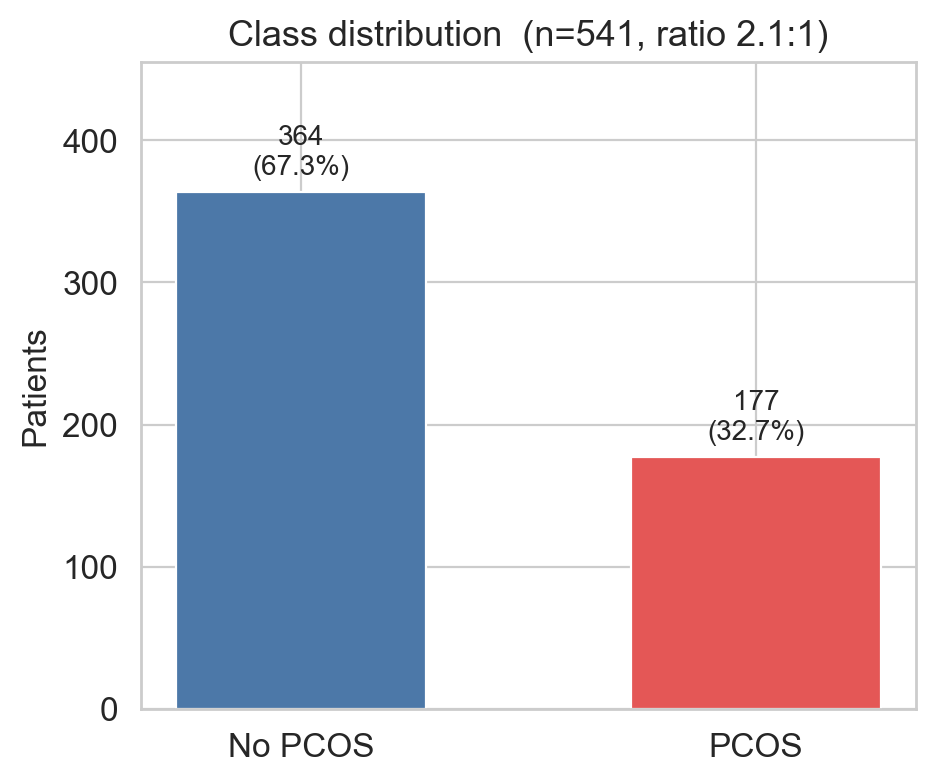
\includegraphics[width=\textwidth]{reports/figures/01_class_balance.png}
  \caption{Class distribution (541 patients)}
\end{subfigure}\hfill
\begin{subfigure}[b]{0.31\textwidth}
  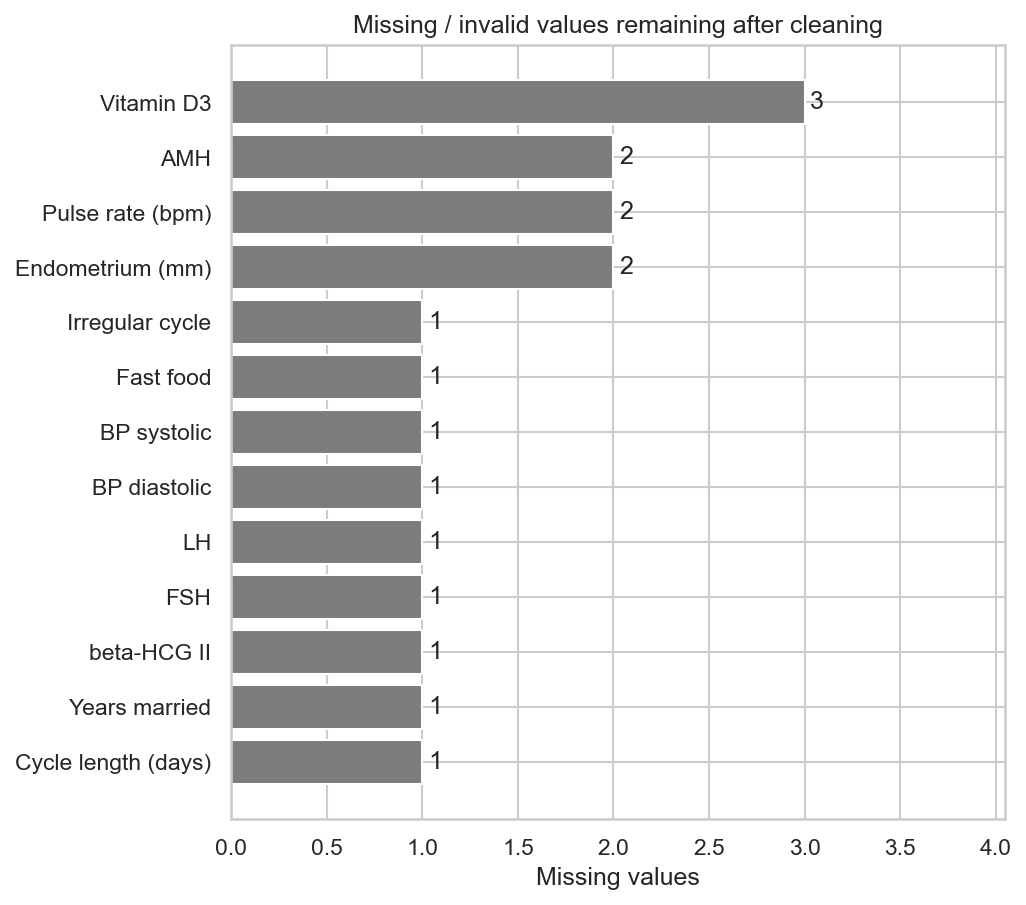
\includegraphics[width=\textwidth]{reports/figures/02_missingness.png}
  \caption{Missing value profile ($<$1\% per feature)}
\end{subfigure}\hfill
\begin{subfigure}[b]{0.35\textwidth}
  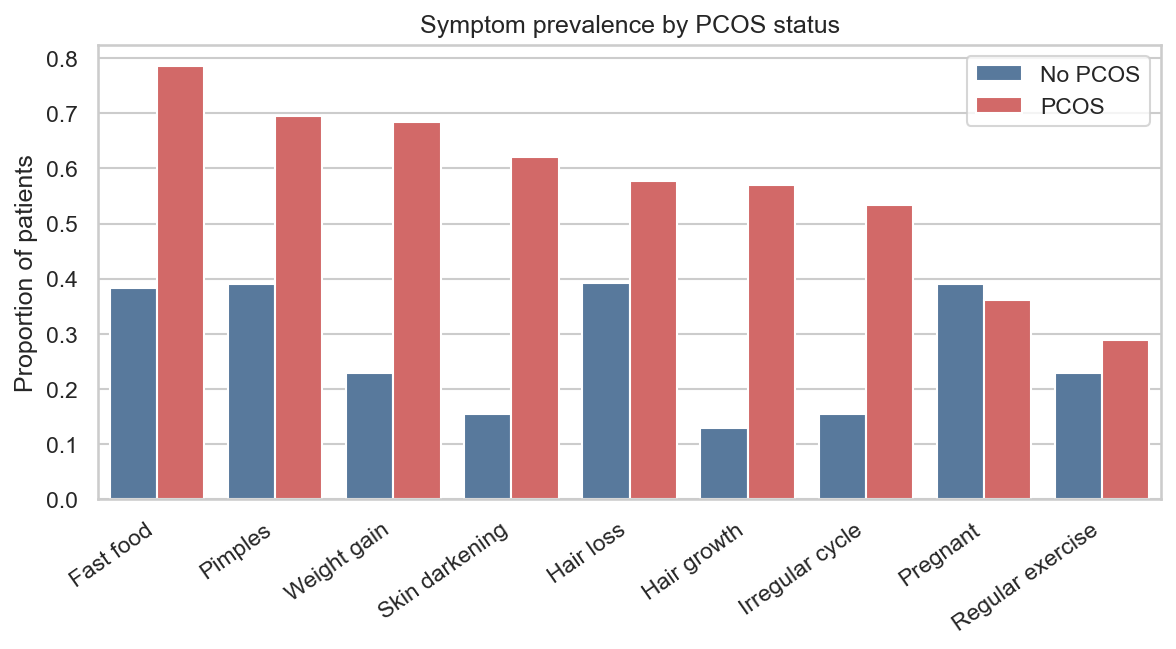
\includegraphics[width=\textwidth]{reports/figures/06_symptom_prevalence.png}
  \caption{Symptom prevalence by class}
\end{subfigure}
\caption{Dataset overview: class balance, missingness, and symptom prevalence.
  The 2.06:1 non-PCOS to PCOS ratio motivates SMOTE balancing.  Binary symptoms show
  substantially higher prevalence in the PCOS group.}
\label{fig:eda}
\end{figure*}

% =============================================================================
\section{EXPLORATORY DATA ANALYSIS}
% =============================================================================

\subsection{Feature Discriminability}
Table~\ref{tab:cohens_d} lists the ten features with the largest absolute Cohen's $d$,
computed from the cleaned dataset before any train/test split.  Follicle counts on both
ovaries dominate with $d > 1.49$, confirming that the Rotterdam ultrasound criterion
carries most of the classification signal in this cohort.  Skin darkening, hair growth,
and weight gain follow at $d \approx 1.0$, representing the hyperandrogenism symptom cluster.
Importantly, FSH, LH, TSH, prolactin, and blood pressure show near-zero separation
($d < 0.18$), suggesting that the expensive endocrine panel contributes minimally to
classification — a finding quantified in Section~\ref{sec:tiers}.

\begin{table}[t]
\centering
\caption{Top discriminating features (Cohen's $d$, verified from \texttt{summary\_statistics.csv}).}
\label{tab:cohens_d}
\small
\begin{tabular}{lcc}
\toprule
\textbf{Feature} & \textbf{Cohen's $d$} & \textbf{Direction} \\
\midrule
Follicle count (R) & 1.702 & Higher $\to$ PCOS \\
Follicle count (L) & 1.493 & Higher $\to$ PCOS \\
Skin darkening     & 1.091 & Higher $\to$ PCOS \\
Hair growth        & 1.042 & Higher $\to$ PCOS \\
Weight gain        & 1.026 & Higher $\to$ PCOS \\
Fast food          & 0.893 & Higher $\to$ PCOS \\
Irregular cycle    & 0.871 & Higher $\to$ PCOS \\
Pimples            & 0.641 & Higher $\to$ PCOS \\
AMH                & 0.543 & Higher $\to$ PCOS \\
Weight (kg)        & 0.446 & Higher $\to$ PCOS \\
\bottomrule
\end{tabular}
\end{table}

\subsection{Follicle Count Separation}
The right-ovary follicle count shows the strongest class separation in the dataset:
mean $10.76$ in PCOS versus $4.64$ in non-PCOS (Cohen's $d = 1.70$; Fig.~\ref{fig:eda2}).
The left ovary shows a similar pattern ($d = 1.49$).  This aligns with the Rotterdam
morphological criterion (polycystic ovarian morphology defined as $\geq 12$ follicles) and
is reflected directly in SHAP global feature importance (Section~\ref{sec:shap}).

\begin{figure*}[t]
\centering
\begin{subfigure}[b]{0.31\textwidth}
  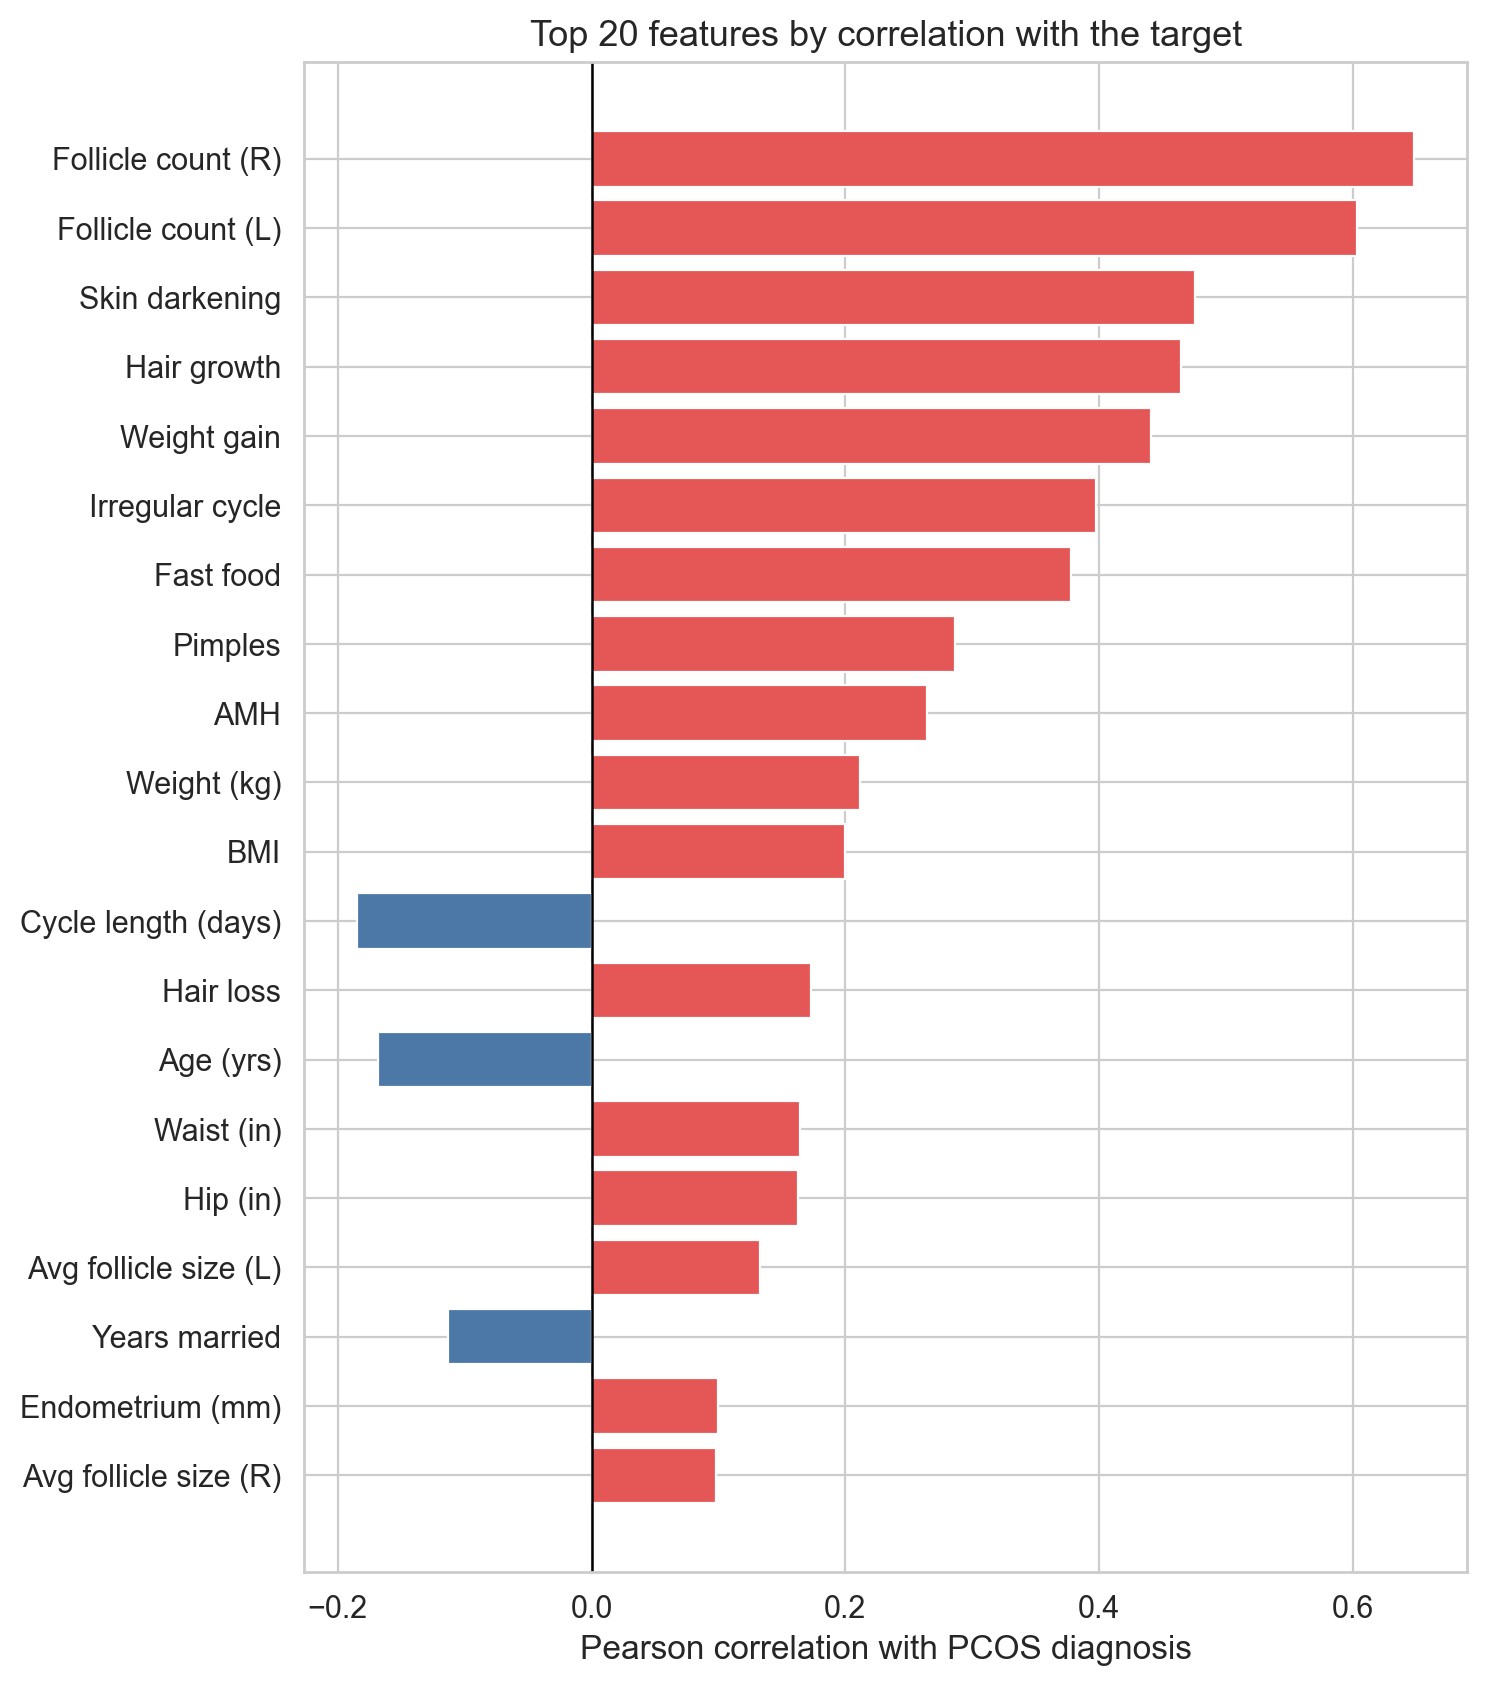
\includegraphics[width=\textwidth]{reports/figures/03_target_correlations.png}
  \caption{Absolute correlation with PCOS target}
\end{subfigure}\hfill
\begin{subfigure}[b]{0.35\textwidth}
  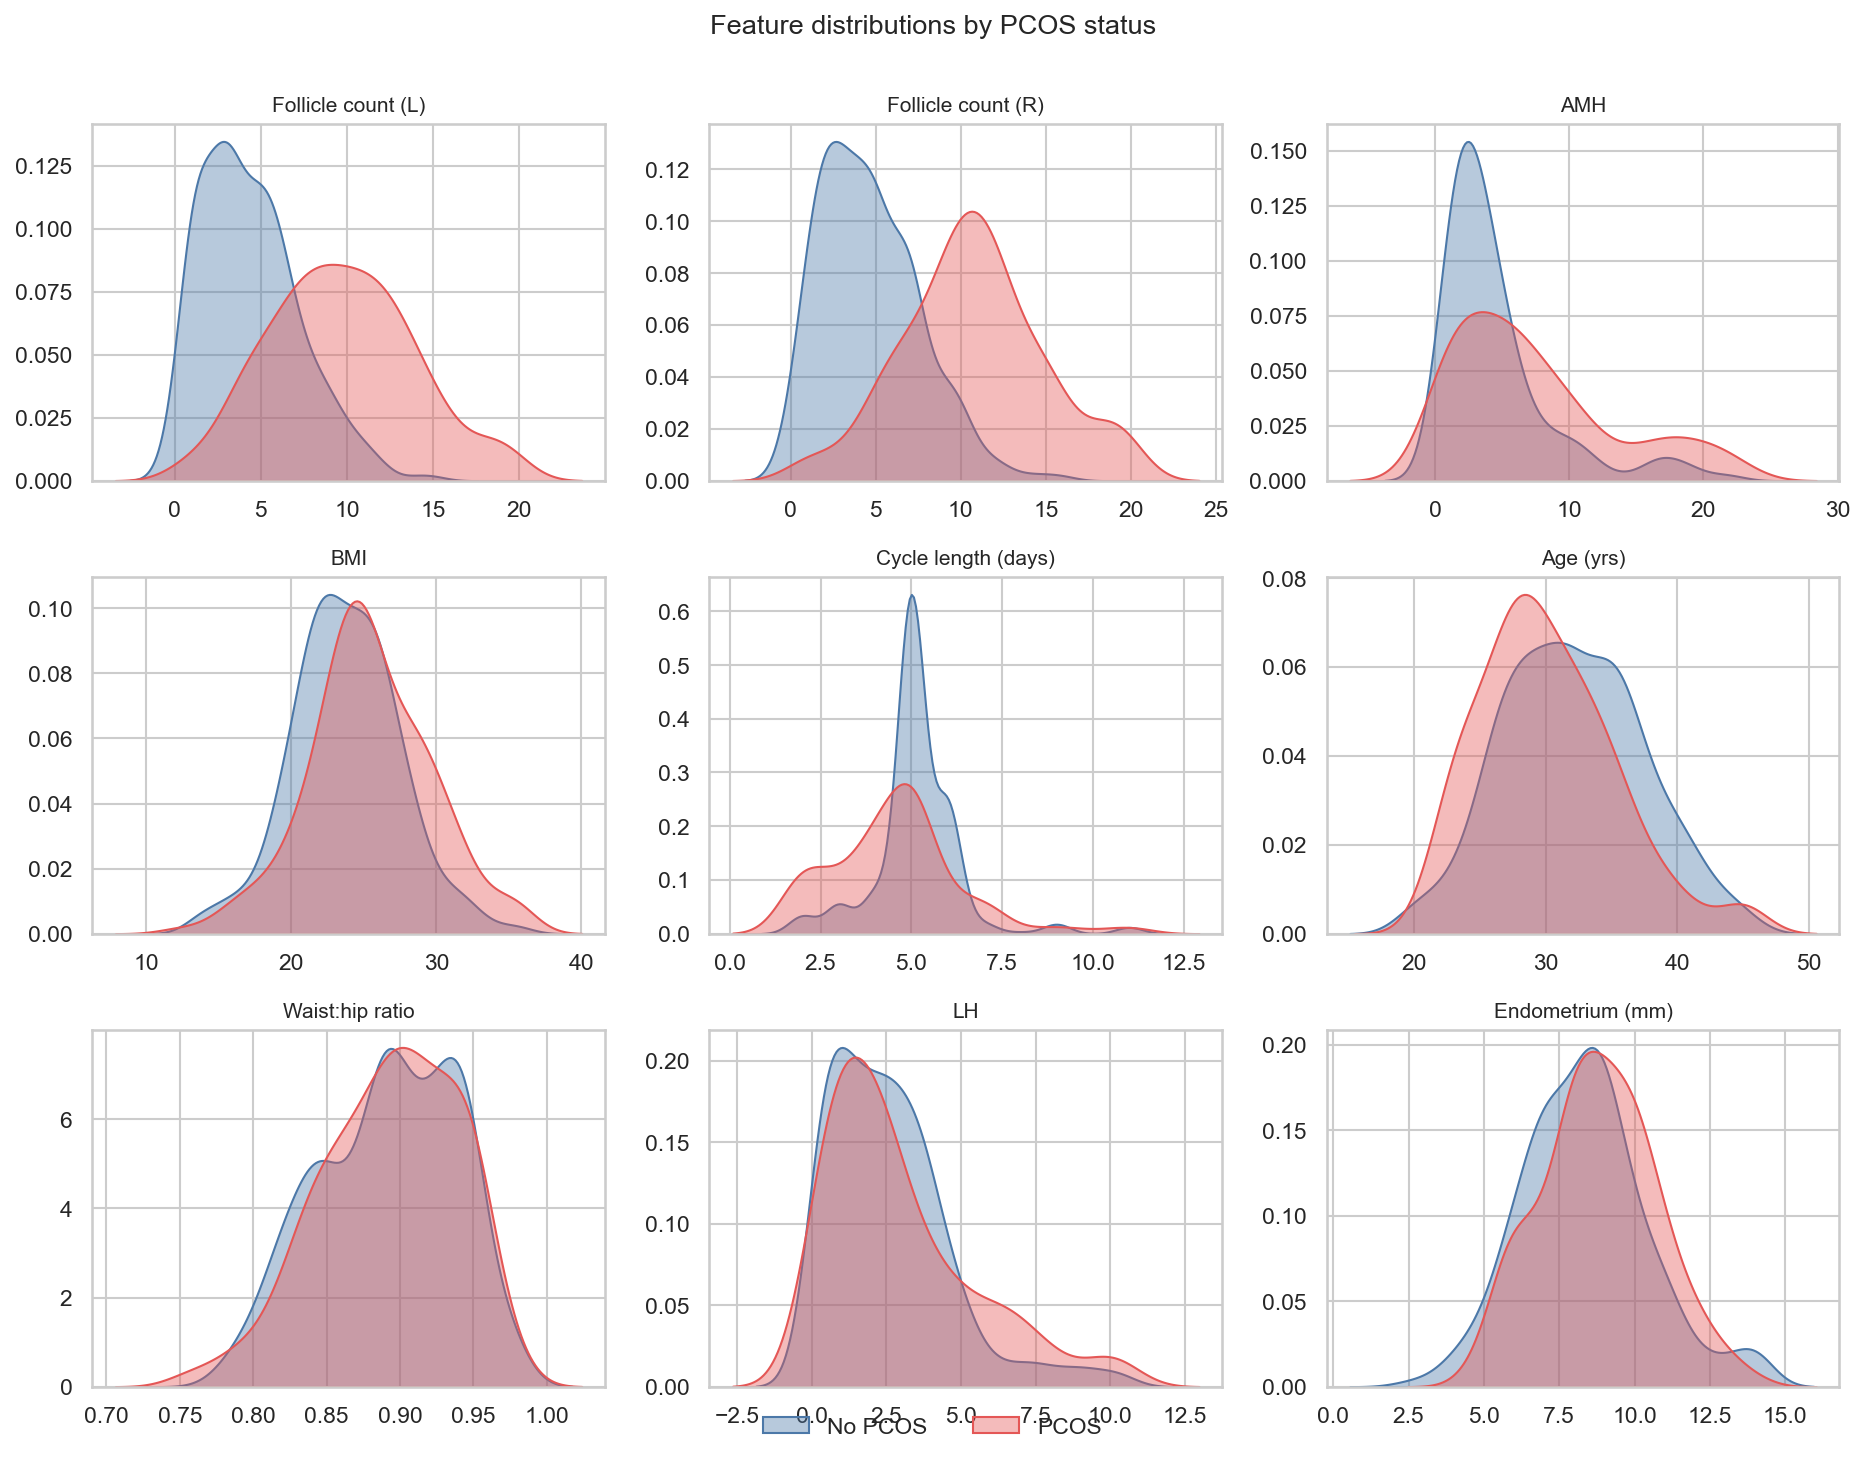
\includegraphics[width=\textwidth]{reports/figures/05_key_distributions.png}
  \caption{Distribution of top features by class}
\end{subfigure}\hfill
\begin{subfigure}[b]{0.31\textwidth}
  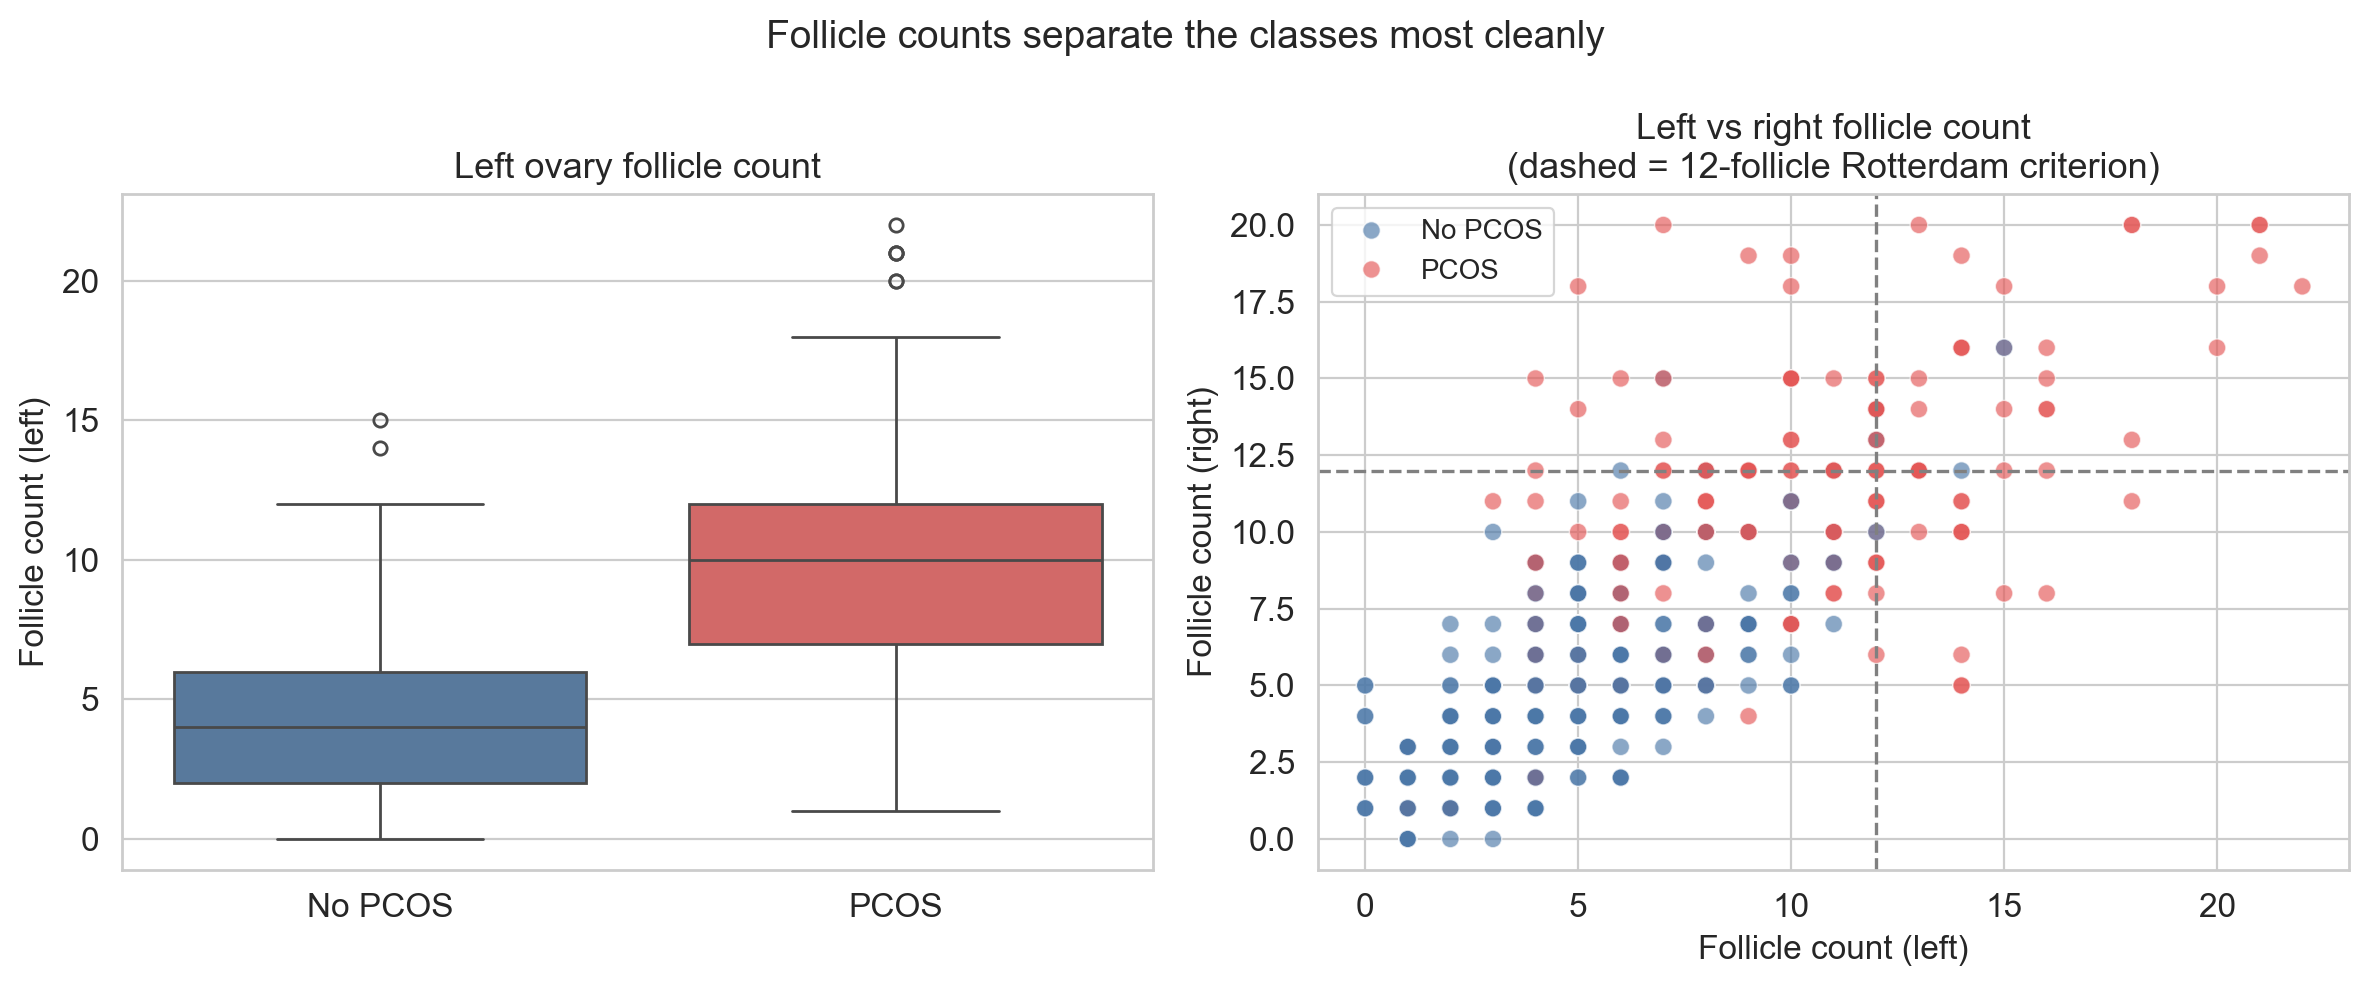
\includegraphics[width=\textwidth]{reports/figures/07_follicle_separation.png}
  \caption{Follicle count class separation ($d = 1.70$)}
\end{subfigure}
\caption{Feature discriminability: target correlations, key feature distributions,
  and follicle count class separation.  The Rotterdam morphological criterion
  (follicles $\geq 12$) is clearly visible as a natural decision boundary.}
\label{fig:eda2}
\end{figure*}

\begin{figure*}[t]
\centering
\begin{subfigure}[b]{0.48\textwidth}
  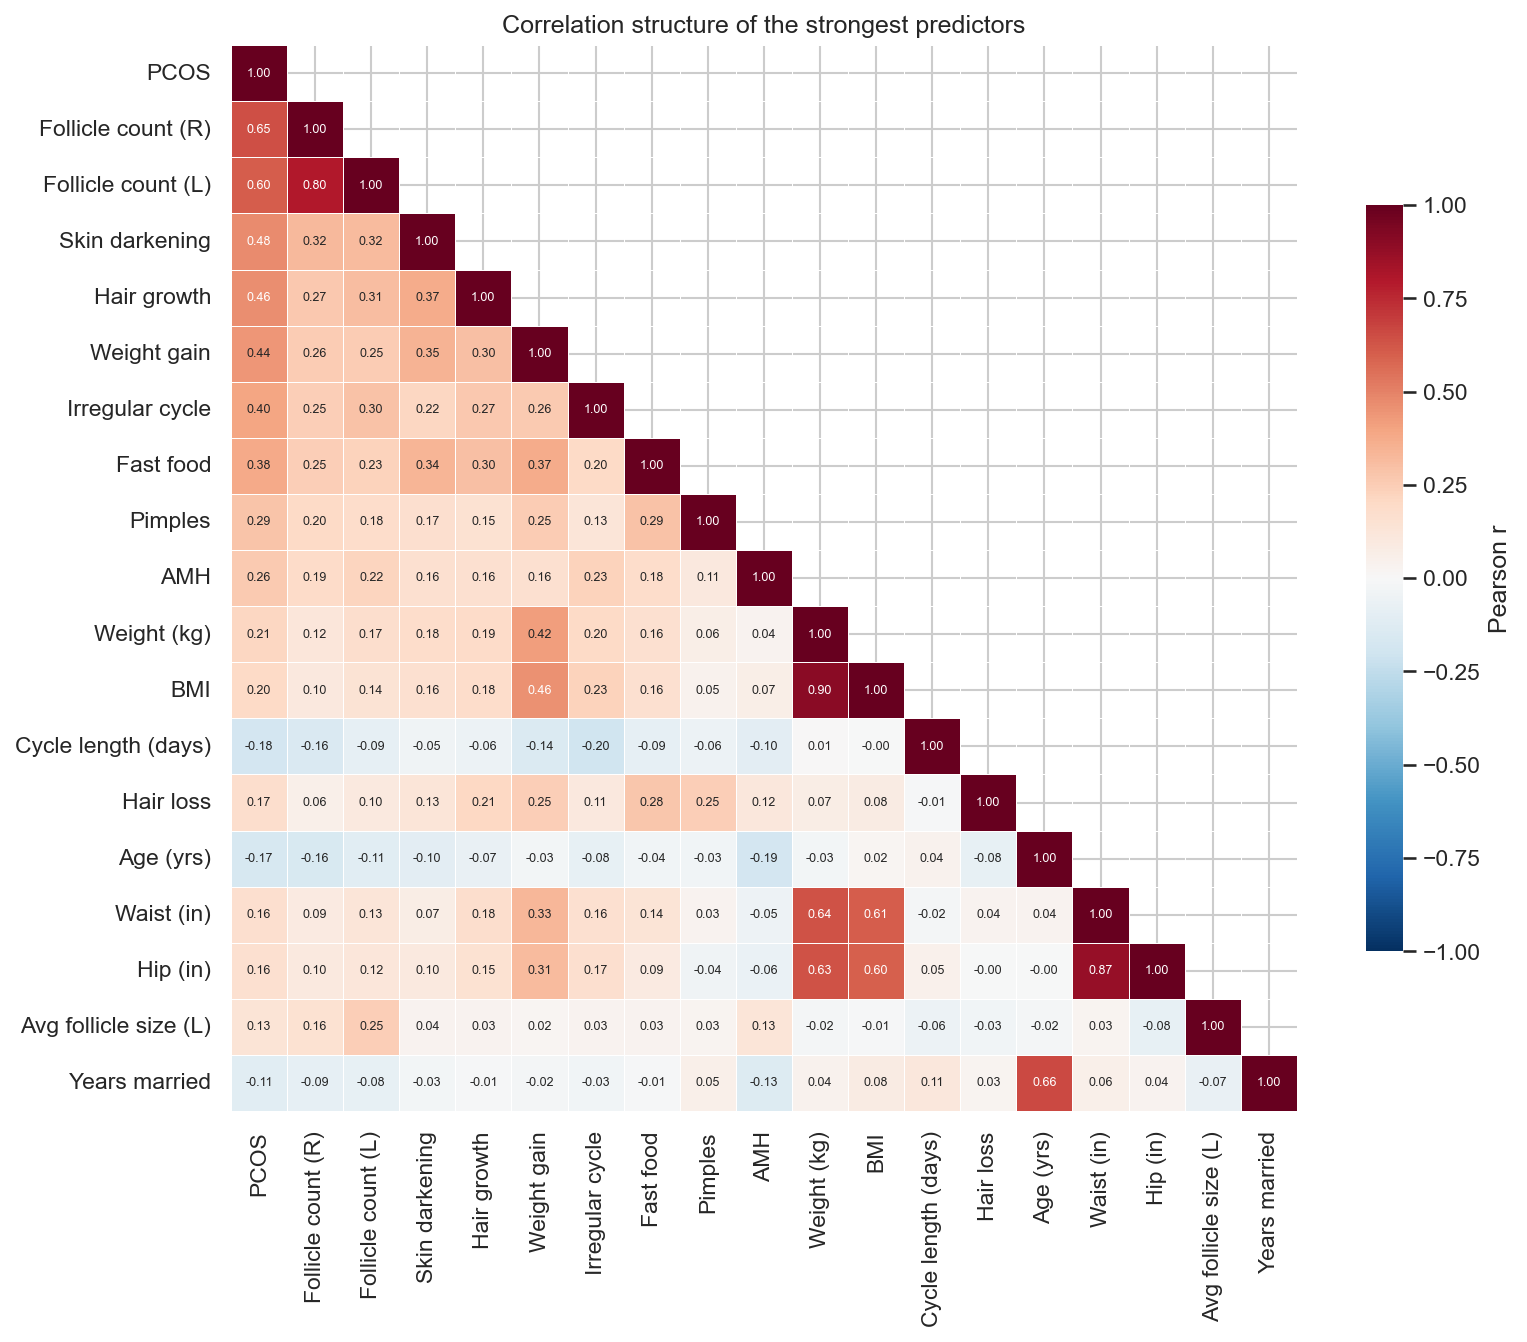
\includegraphics[width=\textwidth]{reports/figures/04_correlation_heatmap.png}
  \caption{Inter-feature correlation heatmap}
\end{subfigure}\hfill
\begin{subfigure}[b]{0.48\textwidth}
  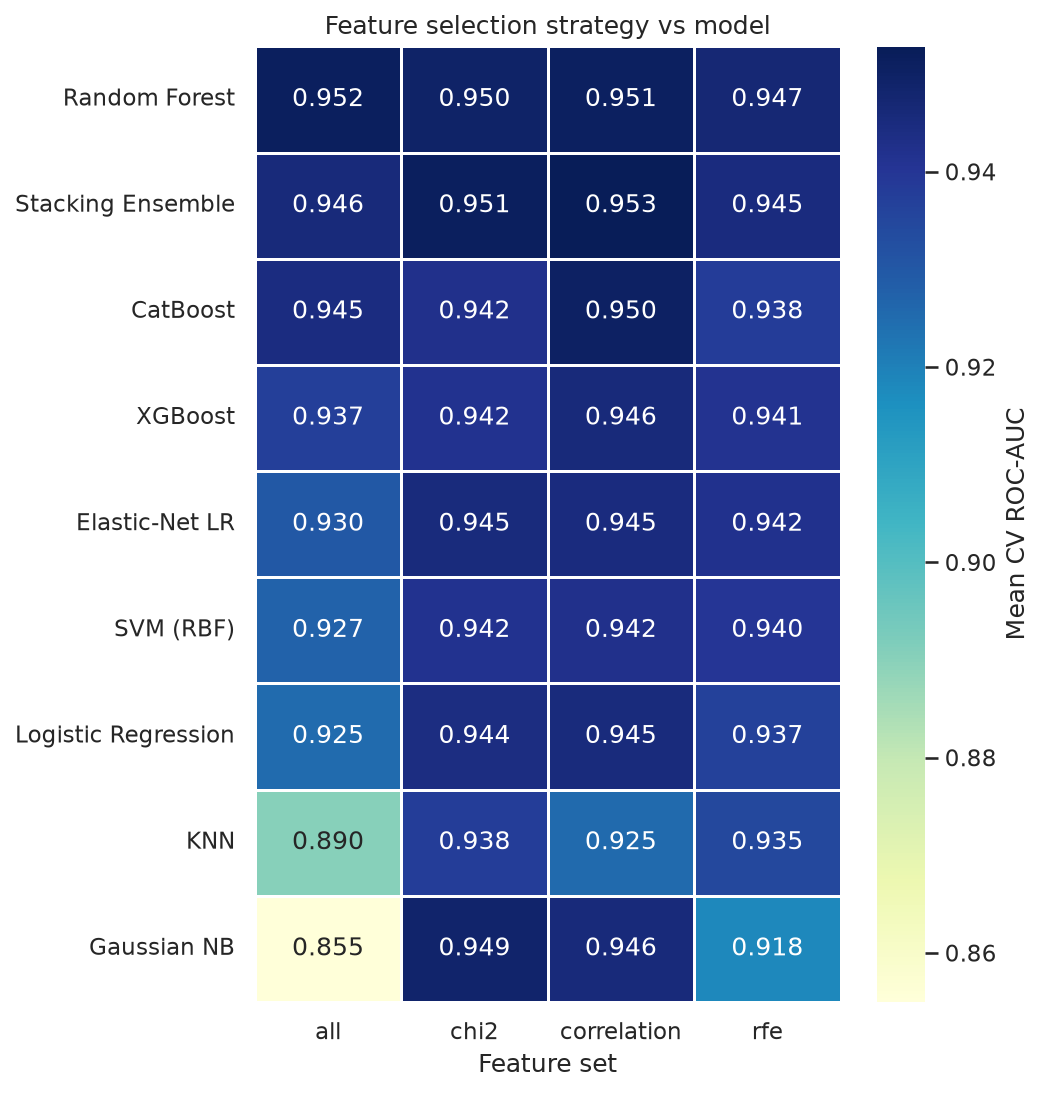
\includegraphics[width=\textwidth]{reports/figures/09_feature_set_comparison.png}
  \caption{Feature selection method comparison (CV ROC-AUC)}
\end{subfigure}
\caption{Feature correlation structure and feature selection results.
  The correlation heatmap motivates the redundancy-removal step in the
  correlation selector.  All three selection strategies outperform the
  all-features baseline by 0.015--0.022 AUC.}
\label{fig:correlations}
\end{figure*}

% =============================================================================
\section{METHODOLOGY}
% =============================================================================

\subsection{Train/Test Split}
The full 541-patient cohort was split once, stratified by the PCOS label, with 80\%
(432 patients) assigned to the training/validation pool and 20\% (109 patients: 73
non-PCOS, 36 PCOS) held out as an untouched test set.  All model selection, feature-set
comparison, and hyperparameter choices use only the training pool.  The test set was
evaluated exactly once, at the end.  Random seed: 42.

\subsection{Cross-Validation}
Model selection uses repeated stratified 10-fold cross-validation with 3 repeats,
producing 30 fold scores per model (CV folds $\times$ repeats = $10 \times 3$).
Stratification preserves the 2.06:1 class ratio within each fold.  The full
preprocessing pipeline (impute $\to$ scale/encode $\to$ select $\to$ SMOTE $\to$ classify)
is refit independently on each training fold, so no information from validation
data influences any fitted step.

\subsection{Machine Learning Models}
Nine classifiers were compared, spanning the useful hypothesis space for tabular
clinical data (Table~\ref{tab:models}).  Base classifiers for the stacking ensemble are
Logistic Regression, Random Forest, SVM (RBF), and XGBoost, with a Logistic Regression
meta-learner trained on 5-fold out-of-fold predicted probabilities.
CatBoost \cite{prokhorenkova2018catboost} is included specifically to reproduce Paper 3's
reported 95.7\% accuracy under the same evaluation protocol.
The deep-learning architectures in Paper 4 (CNN, RNN, LSTM, Bi-LSTM) are structurally
inapplicable to static tabular data and were intentionally excluded.

\begin{table}[t]
\centering
\caption{Models and key configuration.}
\label{tab:models}
\small
\begin{tabular}{lp{4.0cm}}
\toprule
\textbf{Model} & \textbf{Key Configuration} \\
\midrule
Logistic Regression   & \texttt{solver=liblinear}, \texttt{max\_iter=5000} \\
Elastic-Net LR        & \texttt{penalty=elasticnet}, \texttt{l1\_ratio=0.5}, \texttt{C=1.0} \\
Gaussian Naive Bayes  & Default (strong independence assumption) \\
KNN                   & \texttt{n\_neighbors=11}, \texttt{weights=distance} \\
SVM (RBF)             & \texttt{C=1.0}, \texttt{gamma=scale} \\
Random Forest         & 400 trees, \texttt{min\_samples\_leaf=2} \\
XGBoost               & 400 trees, \texttt{depth=4}, \texttt{lr=0.05} \\
CatBoost              & 400 iters, \texttt{depth=4}, \texttt{lr=0.05} \\
Stacking Ensemble     & Base: LR, RF, SVM, XGBoost; meta: LR \\
\bottomrule
\end{tabular}
\end{table}

\subsection{Feature Selection}
Four feature-set strategies were compared under identical CV folds:

\begin{itemize}[leftmargin=*,topsep=2pt,itemsep=1pt]
  \item \textbf{All features (41):} Baseline — no selection.
  \item \textbf{Correlation (20 features):} Two-pass filter — (1) keep features with
        $|\text{corr}(\text{feature}, y)| \geq 0.10$; (2) from remaining pairs with
        inter-feature correlation $> 0.85$, drop the weaker one.
  \item \textbf{Chi-square (15 features):} \texttt{SelectKBest} with $\chi^2$ statistic
        after non-negative scaling.
  \item \textbf{RFE (15 features):} Recursive Feature Elimination driven by Logistic
        Regression, removing one feature per step.
\end{itemize}

All selectors are implemented as scikit-learn transformers and run inside each CV fold,
preventing selection-leakage.  The 20 features selected by the correlation filter are:
follicle counts (R and L), skin darkening, hair growth, weight gain, irregular cycle,
fast food, AMH, pimples, weight, waist circumference, cycle length, hair loss, age,
average follicle sizes (R and L), years married, endometrium, pulse rate, and LH.

\subsection{Evaluation Metrics}
Primary metric is ROC-AUC, computed from predicted class probabilities.  Secondary
metrics are accuracy, precision ($P = \text{TP}/(\text{TP}+\text{FP})$), recall/sensitivity
($R = \text{TP}/(\text{TP}+\text{FN})$), F1-score ($F1 = 2PR/(P+R)$), specificity
($= \text{TN}/(\text{TN}+\text{FP})$), Brier score, and Expected Calibration Error (ECE).
For the held-out test set, 95\% bootstrap confidence intervals (2000 resamples) are
reported for every metric.  Paired $t$-tests across identical fold scores compare
each model to the reference, with a practical-significance threshold of $\Delta\,\text{AUC} > 0.02$.

% =============================================================================
\section{EXPERIMENTAL RESULTS}
% =============================================================================

\subsection{Cross-Validated Model Comparison}
Table~\ref{tab:cv_results} reports mean CV performance across all models using the
correlation feature set (20 features, best-performing selector).

\begin{table}[t]
\centering
\caption{Cross-validated performance (correlation feature set, 10-fold $\times$ 3 repeats).
  Ordered by CV ROC-AUC.  Verified from \texttt{cv\_results.csv}.}
\label{tab:cv_results}
\small
\begin{tabular}{lcc}
\toprule
\textbf{Model} & \textbf{CV AUC} & \textbf{CV Accuracy} \\
\midrule
\textbf{Random Forest}  & $\mathbf{0.957 \pm 0.017}$ & $0.891 \pm 0.025$ \\
Stacking Ensemble       & $0.951 \pm 0.020$           & $0.896 \pm 0.034$ \\
Gaussian NB             & $0.951 \pm 0.023$           & $0.864 \pm 0.045$ \\
Elastic-Net LR          & $0.948 \pm 0.016$           & $0.889 \pm 0.026$ \\
Logistic Regression     & $0.947 \pm 0.017$           & $0.880 \pm 0.035$ \\
XGBoost                 & $0.944 \pm 0.018$           & $0.887 \pm 0.040$ \\
SVM (RBF)               & $0.939 \pm 0.022$           & $0.882 \pm 0.054$ \\
KNN                     & $0.929 \pm 0.037$           & $0.873 \pm 0.044$ \\
\bottomrule
\end{tabular}
\end{table}

\textbf{No clearly best algorithm.}
Paired $t$-tests across the 30 CV fold scores (Table~\ref{tab:significance}) show that
only KNN differs from Random Forest by a practically meaningful margin
($\Delta = -0.028$, practically separable).  Every other gap is $\leq 0.018$ AUC ---
roughly the fold-to-fold standard deviation ($\sigma = 0.017$).  Several gaps are
statistically significant (e.g., SVM, $p = 0.028$, $\Delta = -0.017$) yet clinically
irrelevant.  Statistical and practical separability disagree for six of eight
comparisons.

\begin{table}[t]
\centering
\caption{Pairwise significance vs.\ Random Forest reference.
  Verified from \texttt{significance\_tests.csv}.
  Practical threshold: $\Delta > 0.020$.}
\label{tab:significance}
\small
\begin{tabular}{lcccc}
\toprule
\textbf{Model} & \textbf{$\Delta$ AUC} & \textbf{$p$} & \textbf{Stat.} & \textbf{Prac.} \\
\midrule
Stacking Ens.  & $-0.006$ & 0.075 & no  & no  \\
Gaussian NB    & $-0.006$ & 0.271 & no  & no  \\
Elastic-Net LR & $-0.009$ & 0.037 & yes & no  \\
LR             & $-0.009$ & 0.041 & yes & no  \\
XGBoost        & $-0.013$ & 0.025 & yes & no  \\
SVM (RBF)      & $-0.017$ & 0.028 & yes & no  \\
KNN            & $-0.028$ & 0.051 & no  & \textbf{yes} \\
\bottomrule
\end{tabular}
\end{table}

\begin{figure*}[t]
\centering
\begin{subfigure}[b]{0.32\textwidth}
  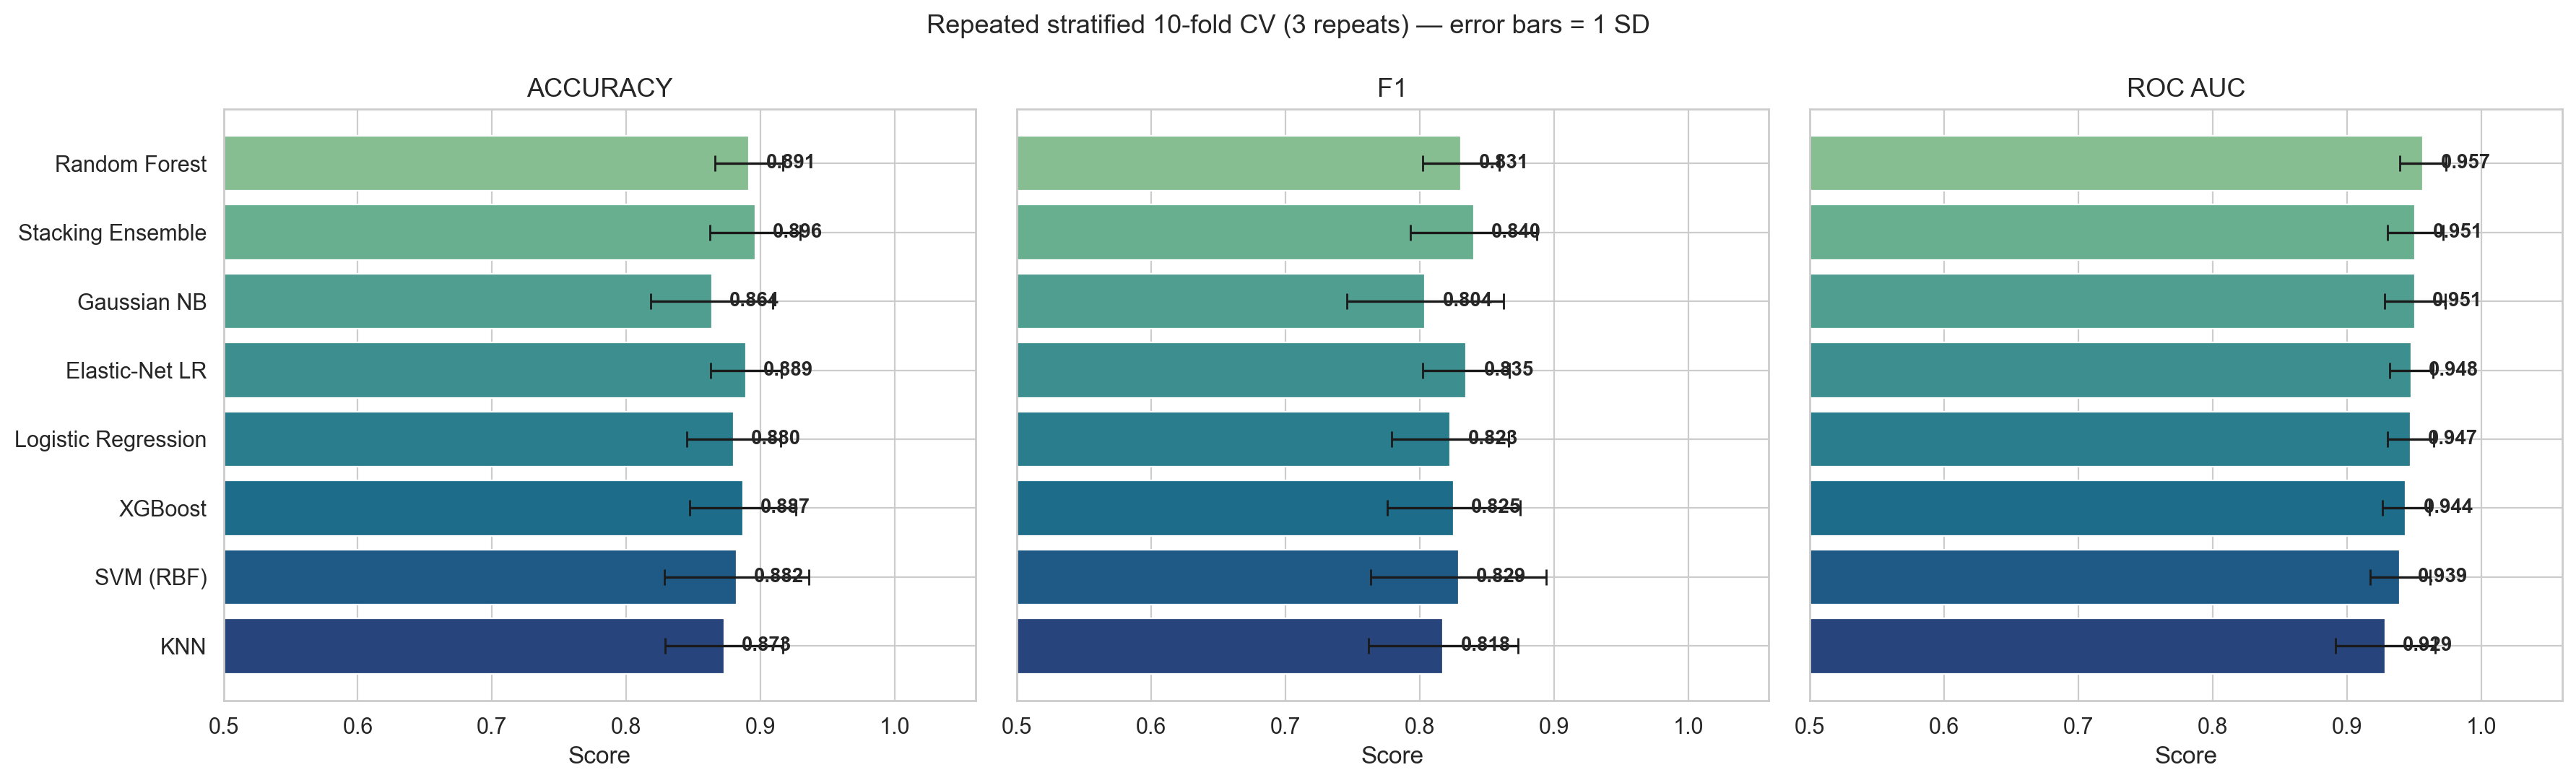
\includegraphics[width=\textwidth]{reports/figures/08_cv_model_comparison.png}
  \caption{CV ROC-AUC comparison (30 fold scores)}
\end{subfigure}\hfill
\begin{subfigure}[b]{0.32\textwidth}
  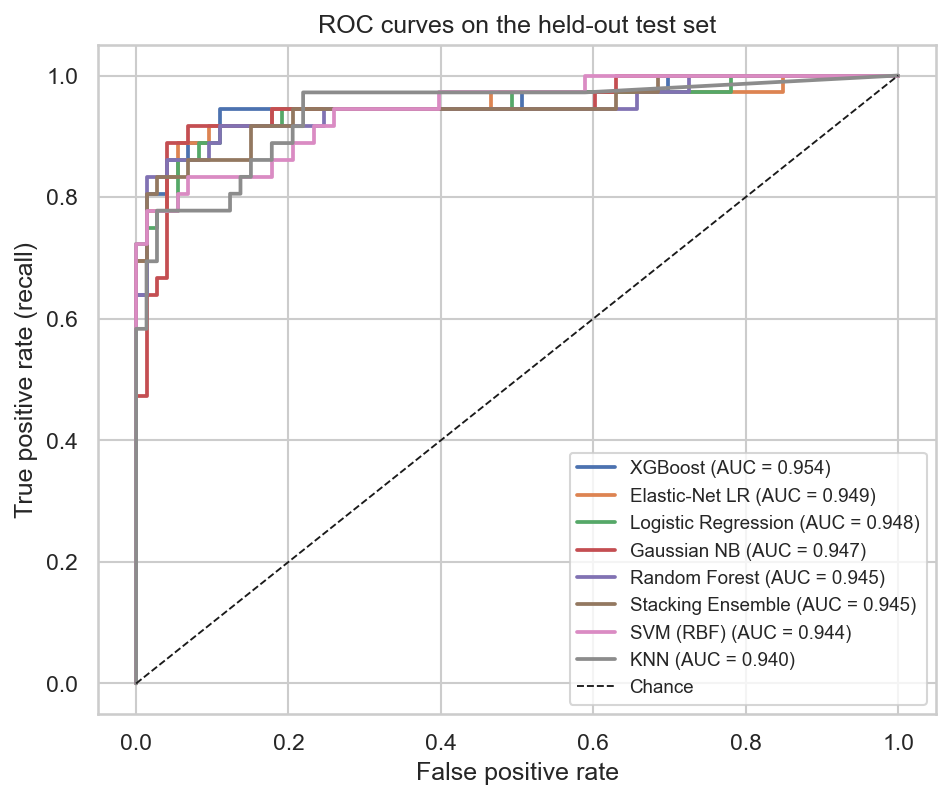
\includegraphics[width=\textwidth]{reports/figures/10_roc_curves.png}
  \caption{Held-out test ROC curves}
\end{subfigure}\hfill
\begin{subfigure}[b]{0.32\textwidth}
  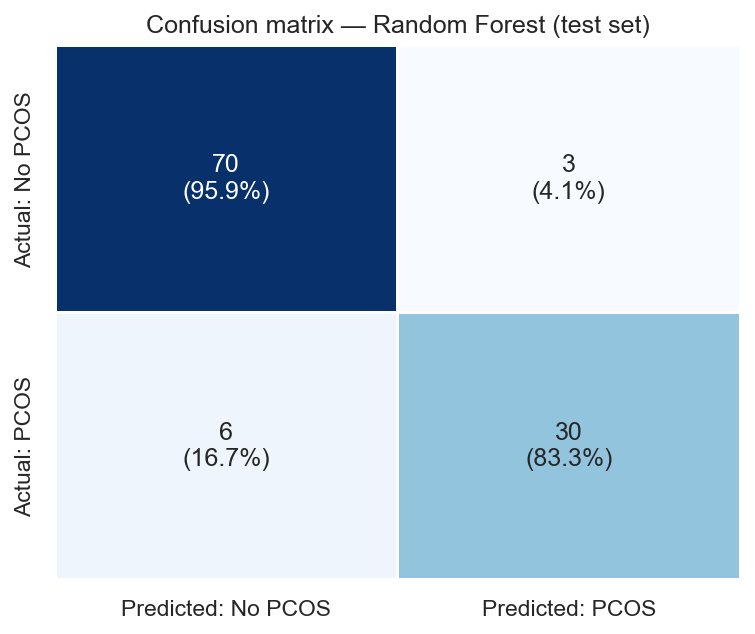
\includegraphics[width=\textwidth]{reports/figures/12_confusion_matrix.png}
  \caption{Confusion matrix (Random Forest)}
\end{subfigure}
\caption{Model comparison, ROC curves, and held-out test confusion matrix.
  RF detects 30 of 36 PCOS cases (TP), misses 6 (FN), with 3 false alarms (FP)
  and 70 correct non-PCOS identifications (TN).}
\label{fig:model_performance}
\end{figure*}

\subsection{Held-out Test Results}
Table~\ref{tab:test_results} reports held-out test performance evaluated once
on the 109-patient test set, ordered by test ROC-AUC.

\begin{table*}[t]
\centering
\caption{Held-out test performance (109 patients: 73 non-PCOS, 36 PCOS).
  Verified from \texttt{test\_results.csv}.  Ordered by test ROC-AUC.}
\label{tab:test_results}
\small
\begin{tabular}{lccccccc}
\toprule
\textbf{Model} & \textbf{Acc} & \textbf{Prec} & \textbf{Recall} & \textbf{F1} & \textbf{Spec} & \textbf{AUC} & \textbf{AP} \\
\midrule
XGBoost            & 0.927 & 0.912 & 0.861 & 0.886 & 0.959 & 0.954 & 0.944 \\
Elastic-Net LR     & 0.917 & 0.865 & 0.889 & 0.877 & 0.932 & 0.949 & 0.942 \\
Logistic Reg.      & 0.908 & 0.842 & 0.889 & 0.865 & 0.918 & 0.948 & 0.938 \\
Gaussian NB        & 0.908 & 0.825 & 0.917 & 0.868 & 0.904 & 0.947 & 0.926 \\
\textbf{Stacking}  & \textbf{0.927} & \textbf{0.938} & 0.833 & 0.882 & \textbf{0.973} & 0.945 & 0.936 \\
\textbf{Rand. Forest} & 0.917 & 0.909 & 0.833 & 0.870 & 0.959 & 0.945 & 0.938 \\
SVM (RBF)          & 0.899 & 0.879 & 0.806 & 0.841 & 0.945 & 0.944 & 0.927 \\
KNN                & 0.853 & 0.778 & 0.778 & 0.778 & 0.890 & 0.940 & 0.916 \\
\bottomrule
\end{tabular}
\end{table*}

The test ranking differs substantially from the CV ranking (XGBoost ranks 6th in CV,
1st on test; Stacking ranks 2nd in CV, 5th on test), confirming that ranking
uncertainty is large on 109 test patients.
Random Forest and Stacking Ensemble are tied on test AUC ($0.945$); Stacking has
higher precision (0.938) and specificity (0.973), while Gaussian NB has the
highest recall (0.917).

\textbf{Bootstrap confidence intervals (Random Forest, test set):}
Accuracy $0.917$ [CI: $0.862$, $0.963$];
Precision $0.909$ [CI: $0.800$, $1.000$];
Recall $0.833$ [CI: $0.703$, $0.944$];
F1 $0.870$ [CI: $0.781$, $0.946$];
Specificity $0.959$ [CI: $0.904$, $1.000$];
ROC-AUC $0.945$ [CI: $0.887$, $0.991$].

The recall CI width of 0.241 illustrates that a 109-patient test set ---
including only 36 positive cases --- cannot pin down sensitivity to better
than $\pm 12$ percentage points, regardless of the algorithm.

\begin{figure*}[t]
\centering
\begin{subfigure}[b]{0.32\textwidth}
  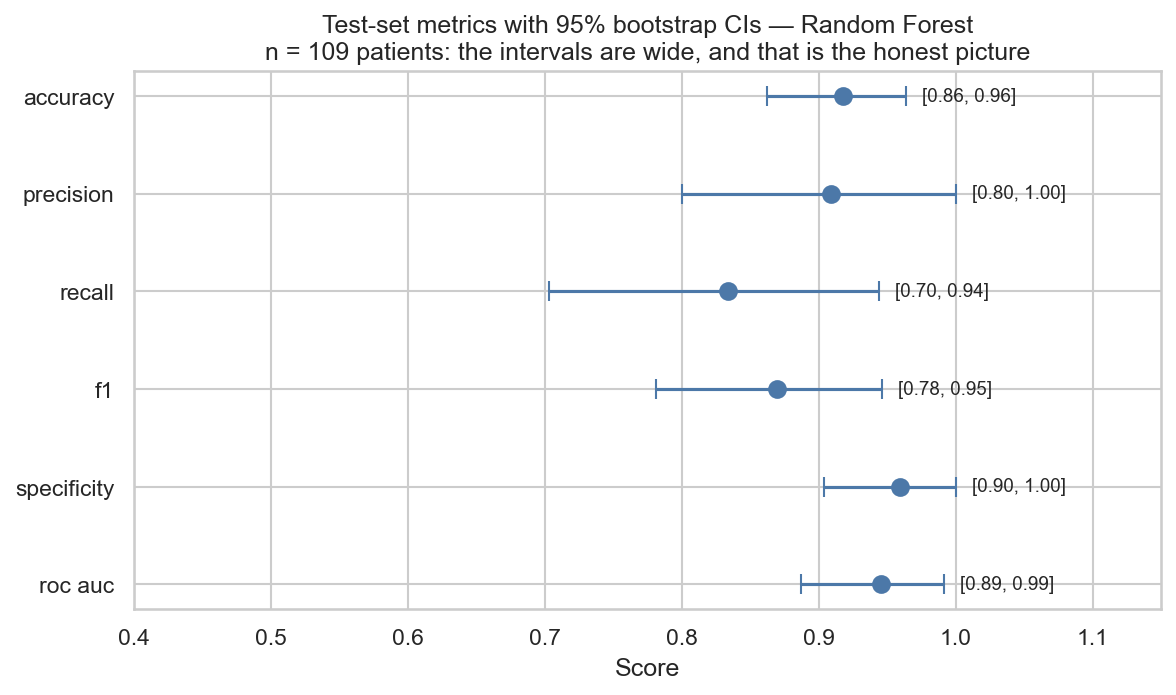
\includegraphics[width=\textwidth]{reports/figures/25_bootstrap_ci.png}
  \caption{95\% bootstrap CIs for all test metrics}
\end{subfigure}\hfill
\begin{subfigure}[b]{0.32\textwidth}
  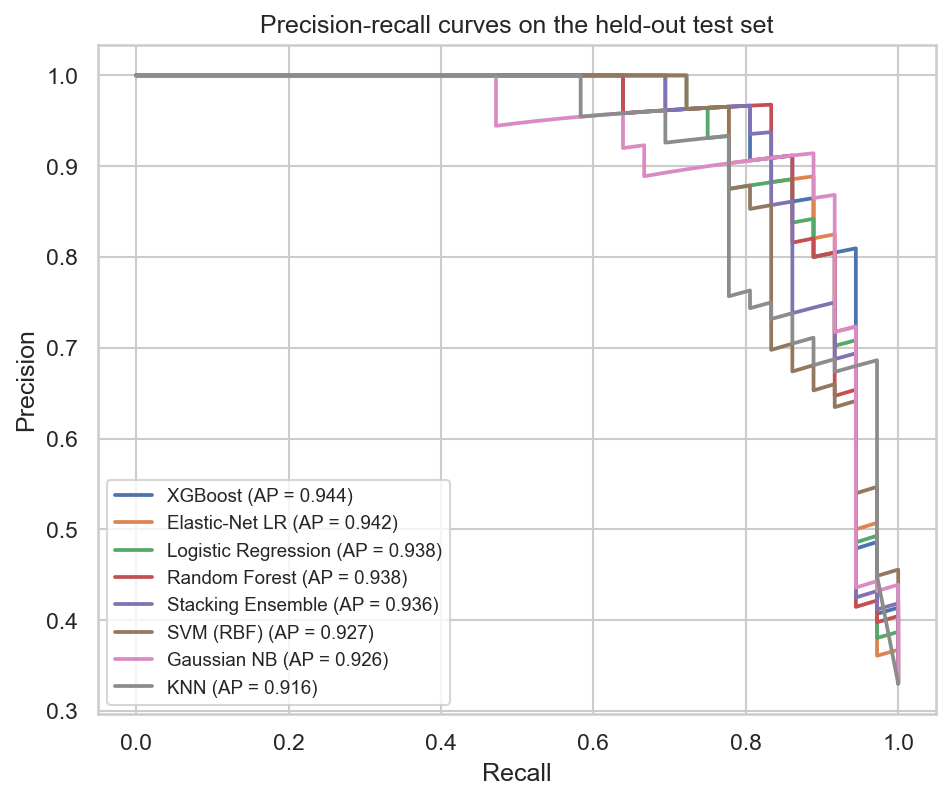
\includegraphics[width=\textwidth]{reports/figures/11_pr_curves.png}
  \caption{Precision-Recall curves (test set)}
\end{subfigure}\hfill
\begin{subfigure}[b]{0.32\textwidth}
  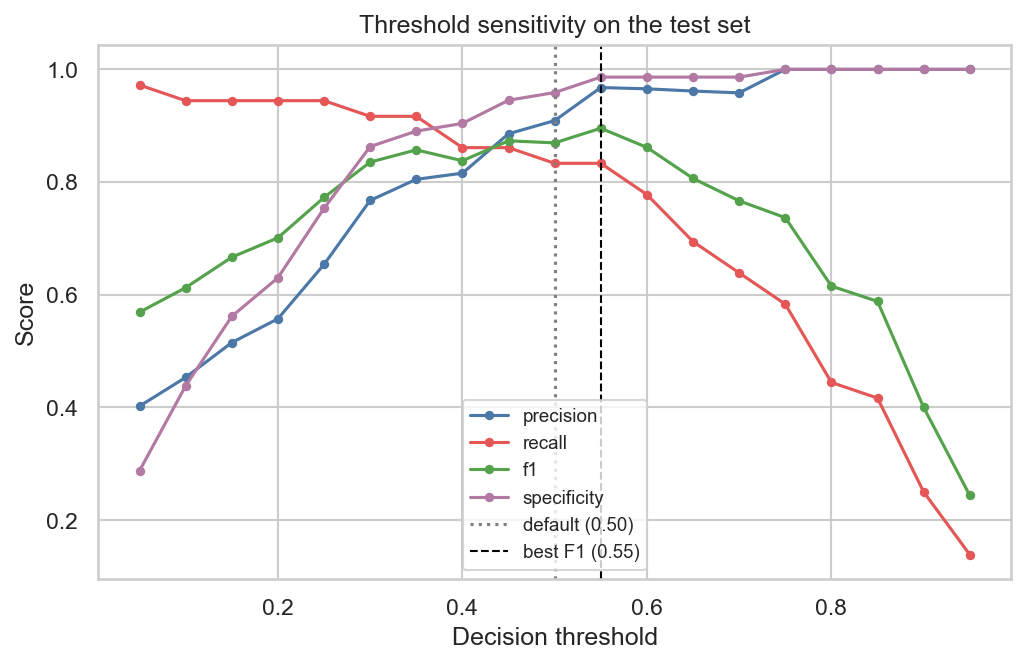
\includegraphics[width=\textwidth]{reports/figures/14_threshold_sweep.png}
  \caption{Threshold sweep: precision vs.\ recall}
\end{subfigure}
\caption{Uncertainty quantification and threshold analysis.
  The wide recall CI ($\pm 12$ points) illustrates the inherent
  imprecision of any single-split evaluation on 36 positive test cases.
  PR curves and threshold analysis guide operating-point selection.}
\label{fig:uncertainty}
\end{figure*}

\subsection{The Leakage Experiment}
\label{sec:leakage}
A critical methodological result: the same pipeline, the same data, and the same folds
were run under two protocols differing only in whether SMOTE and feature selection
execute \emph{before} or \emph{inside} CV folds.

\begin{table}[t]
\centering
\caption{Leakage experiment: correct vs.\ leaky protocol.
  Verified from \texttt{leakage\_experiment.csv}.}
\label{tab:leakage}
\small
\begin{tabular}{lccc}
\toprule
\textbf{Metric} & \textbf{Correct} & \textbf{Leaky} & \textbf{Inflation} \\
\midrule
Accuracy    & 0.900 & 0.927 & $+0.027$ \\
Precision   & 0.856 & 0.923 & $+0.067$ \\
Recall      & 0.836 & 0.934 & $+0.098$ \\
F1          & 0.845 & 0.928 & $+0.083$ \\
ROC-AUC     & 0.949 & 0.975 & $+0.025$ \\
\bottomrule
\end{tabular}
\end{table}

When SMOTE runs before the CV split, synthetic minority samples interpolated from
training-set neighbours can appear in the validation fold --- the model is partially
scored on points derived from its own training data.  When feature selection runs
before the split, the selector reads all 541 labels including those in the validation fold.
This experiment does not prove that all reviewed papers made these mistakes; many do not
describe their protocol in sufficient detail to determine this.  What it does show is
that a 98--99\% accuracy on this 541-row dataset is \emph{reachable through methodology
alone} (Fig.~\ref{fig:leakage_validation}).

\begin{figure*}[t]
\centering
\begin{subfigure}[b]{0.32\textwidth}
  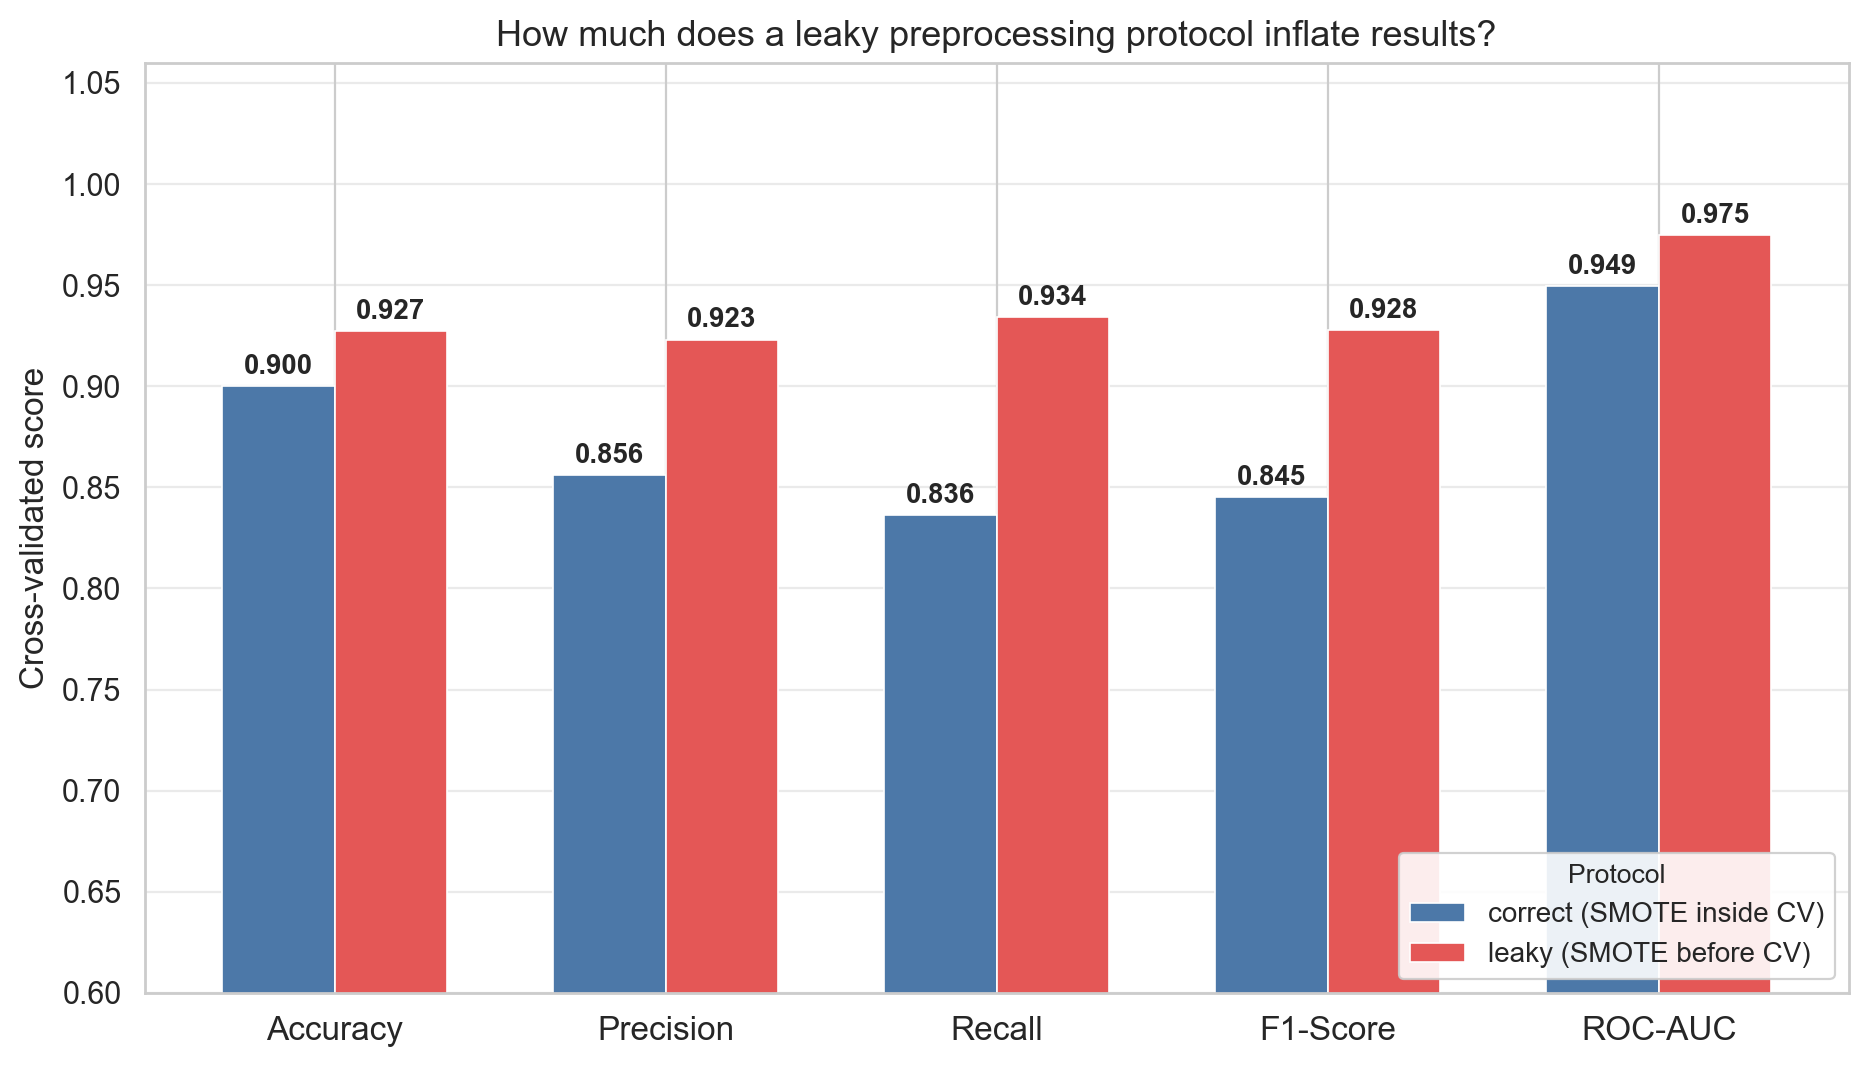
\includegraphics[width=\textwidth]{reports/figures/13_leakage_experiment.png}
  \caption{Leakage inflation (+2.7 pp accuracy, +9.0 pp F1)}
\end{subfigure}\hfill
\begin{subfigure}[b]{0.32\textwidth}
  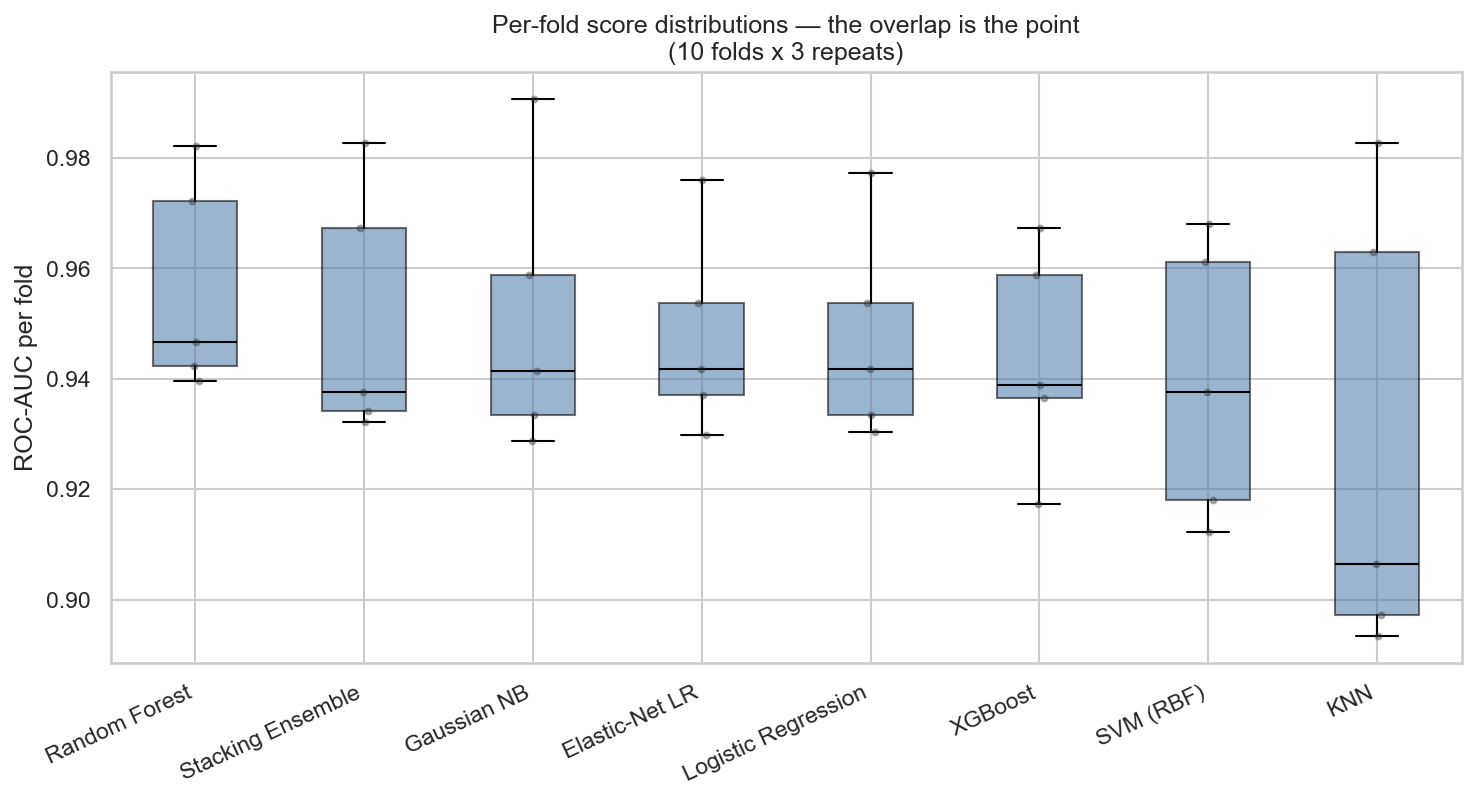
\includegraphics[width=\textwidth]{reports/figures/20_significance_boxplot.png}
  \caption{Paired fold AUC scores (30 folds)}
\end{subfigure}\hfill
\begin{subfigure}[b]{0.32\textwidth}
  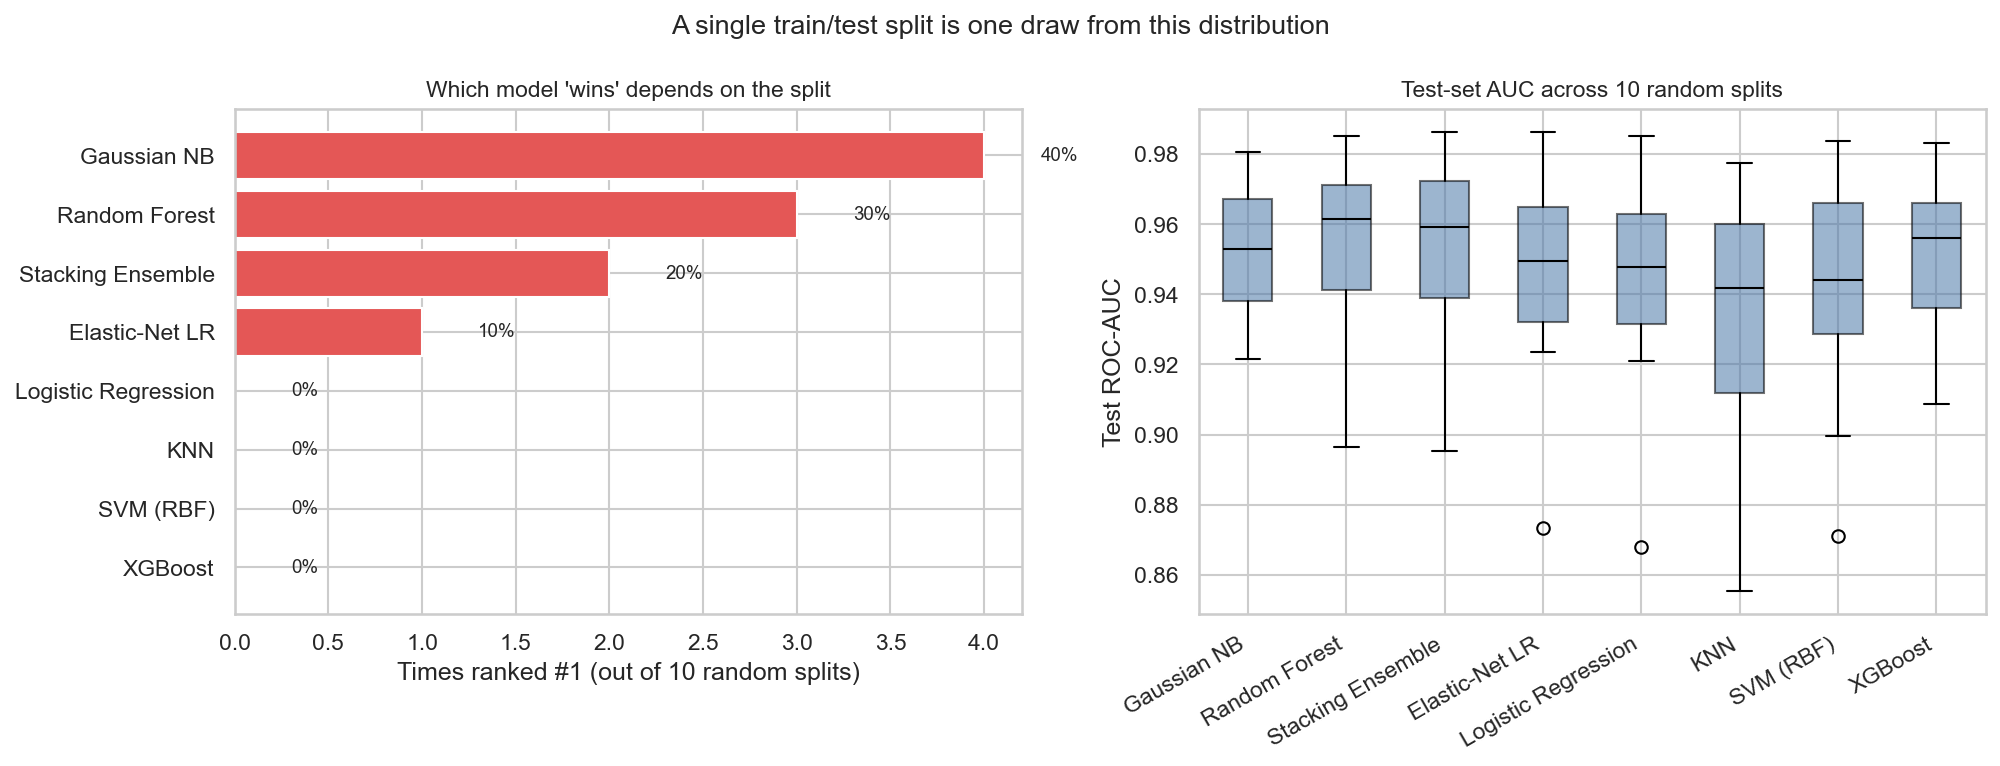
\includegraphics[width=\textwidth]{reports/figures/23_seed_sweep.png}
  \caption{Winner per random seed (10 seeds)}
\end{subfigure}
\caption{Validation rigour: leakage inflation, statistical separability, and
  winner instability across random seeds.  In a 10-seed sweep, 4 distinct
  models win at least once, confirming the absence of a dominant algorithm.}
\label{fig:leakage_validation}
\end{figure*}

\subsection{Feature Selection Comparison}
Table~\ref{tab:feature_sets} compares the four selection strategies.

\begin{table}[t]
\centering
\caption{Feature selection strategy comparison.
  Verified from \texttt{feature\_set\_comparison.csv} (Random Forest baseline).}
\label{tab:feature_sets}
\small
\begin{tabular}{lccc}
\toprule
\textbf{Strategy} & \textbf{Features} & \textbf{CV AUC} & \textbf{Test AUC} \\
\midrule
\textbf{Correlation} & \textbf{20} & \textbf{0.957} & \textbf{0.945} \\
Chi-square           & 15 & 0.952 & 0.945 \\
RFE                  & 15 & 0.952 & 0.945 \\
All features         & 41 & 0.954 & 0.942 \\
\bottomrule
\end{tabular}
\end{table}

All three selectors outperform the all-features baseline on CV AUC.  Correlation and
chi-square are separated by $\approx 0.005$ AUC --- noise on this dataset.
The practical argument reinforces the statistical one: 15--20 measurements are cheaper
to collect in a clinic than 41, with no accuracy cost.

\subsection{Class Imbalance Ablation}
Table~\ref{tab:imbalance} reports the effect of three balancing strategies on the
held-out test set.

\begin{table}[t]
\centering
\caption{Class balancing ablation (held-out test set).
  Verified from \texttt{imbalance\_ablation.csv}.}
\label{tab:imbalance}
\small
\begin{tabular}{lcccc}
\toprule
\textbf{Strategy} & \textbf{Acc} & \textbf{Recall} & \textbf{F1} & \textbf{Spec} \\
\midrule
No balancing   & 0.908 & 0.806 & 0.853 & 0.959 \\
Class weights  & 0.899 & 0.861 & 0.849 & 0.918 \\
\textbf{SMOTE} & \textbf{0.899} & \textbf{0.833} & \textbf{0.845} & \textbf{0.932} \\
\bottomrule
\end{tabular}
\end{table}

No single strategy dominates across all metrics.  SMOTE improves recall over the
no-balancing baseline at the cost of slightly lower specificity.  For a screening
context where false negatives carry higher clinical cost than false positives, this
trade-off is appropriate.

\subsection{Robustness Checks}

\textbf{Nested cross-validation.}
Flat CV (selector chosen on the same data) gives AUC $0.9558$.
Nested CV (selector chosen inside folds) gives AUC $0.9541 \pm 0.020$.
The selection bias is $-0.0017$ --- negligible, because the four feature sets perform
nearly identically (Fig.~\ref{fig:robustness}).

\textbf{AutoML benchmark.}
FLAML (120s budget on the training split) converged on a Random Forest with test
ROC-AUC $0.946$, versus $0.945$ for the hand-built pipeline --- a difference of $+0.0004$.
Accuracy and F1 are \emph{lower} in the AutoML result ($0.899$ vs $0.927$;
$0.831$ vs $0.882$).  The dataset, not the pipeline, is the binding constraint.

\textbf{Seed stability.}
In a 10-seed random-split sweep, 4 of 8 models won at least once.
Gaussian NB won most frequently (40\% of seeds), despite ranking third in CV.
The model's own AUC varies by $0.059$--$0.113$ depending solely on which patients
land in the test set, confirming that any single-split winner ranking is largely noise.

\textbf{Learning curve.}
Validation AUC increases by approximately $+0.0003$ per 100 additional training
patients over the last third of the curve --- essentially flat.  Training AUC
sits at $0.9999$ against a validation plateau of $\approx 0.957$: the model has
saturated what these 41 features can represent.  Additional data would not
substantially improve performance without new feature modalities.

\begin{figure*}[t]
\centering
\begin{subfigure}[b]{0.24\textwidth}
  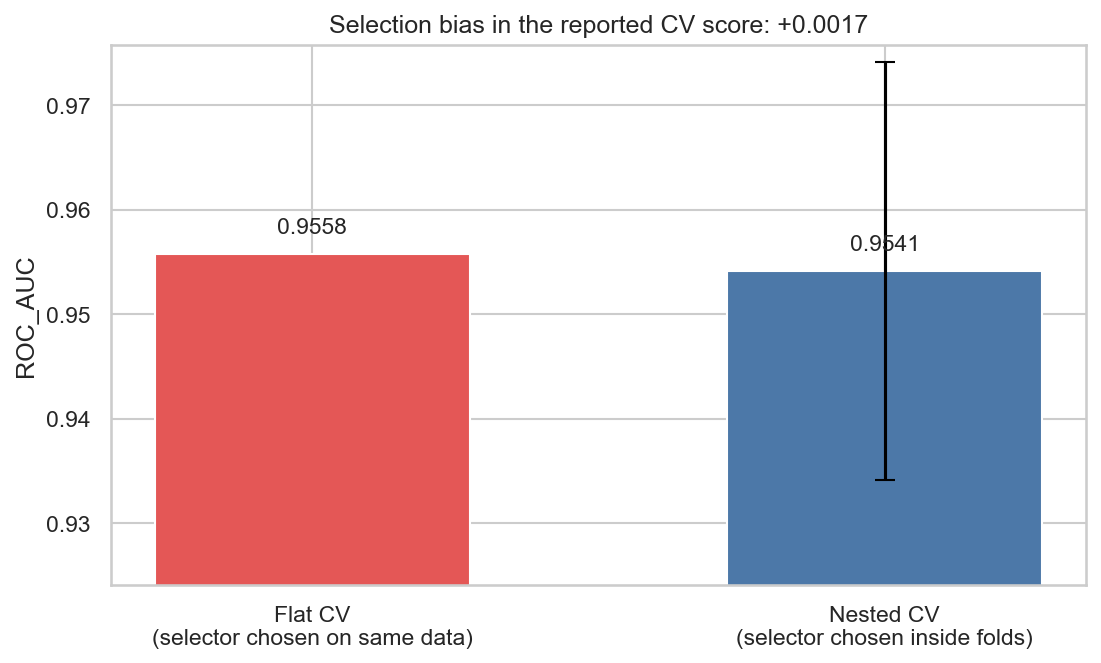
\includegraphics[width=\textwidth]{reports/figures/22_nested_cv.png}
  \caption{Nested vs.\ flat CV AUC}
\end{subfigure}\hfill
\begin{subfigure}[b]{0.24\textwidth}
  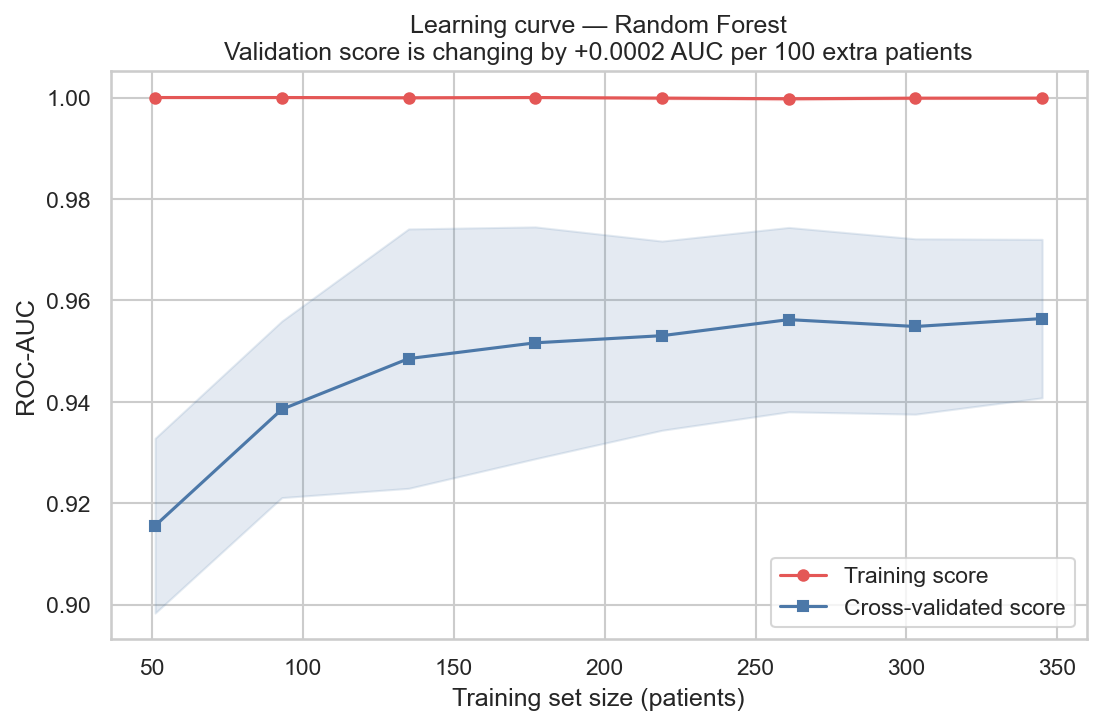
\includegraphics[width=\textwidth]{reports/figures/24_learning_curve.png}
  \caption{Learning curve (AUC vs.\ training size)}
\end{subfigure}\hfill
\begin{subfigure}[b]{0.24\textwidth}
  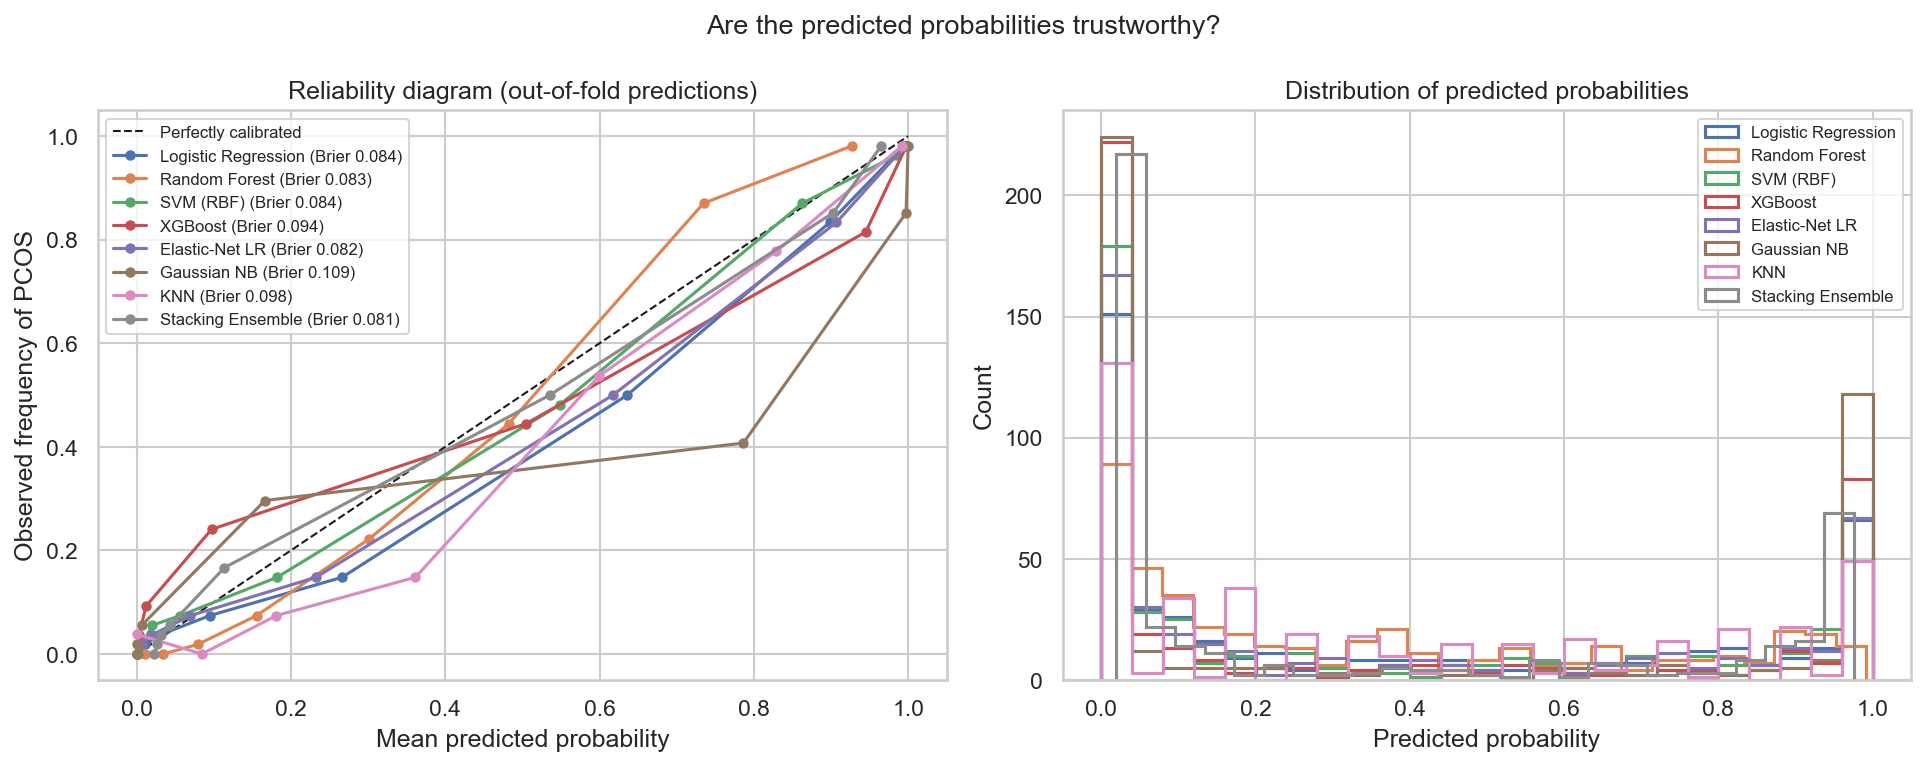
\includegraphics[width=\textwidth]{reports/figures/19_calibration_curves.png}
  \caption{Probability calibration curves}
\end{subfigure}\hfill
\begin{subfigure}[b]{0.24\textwidth}
  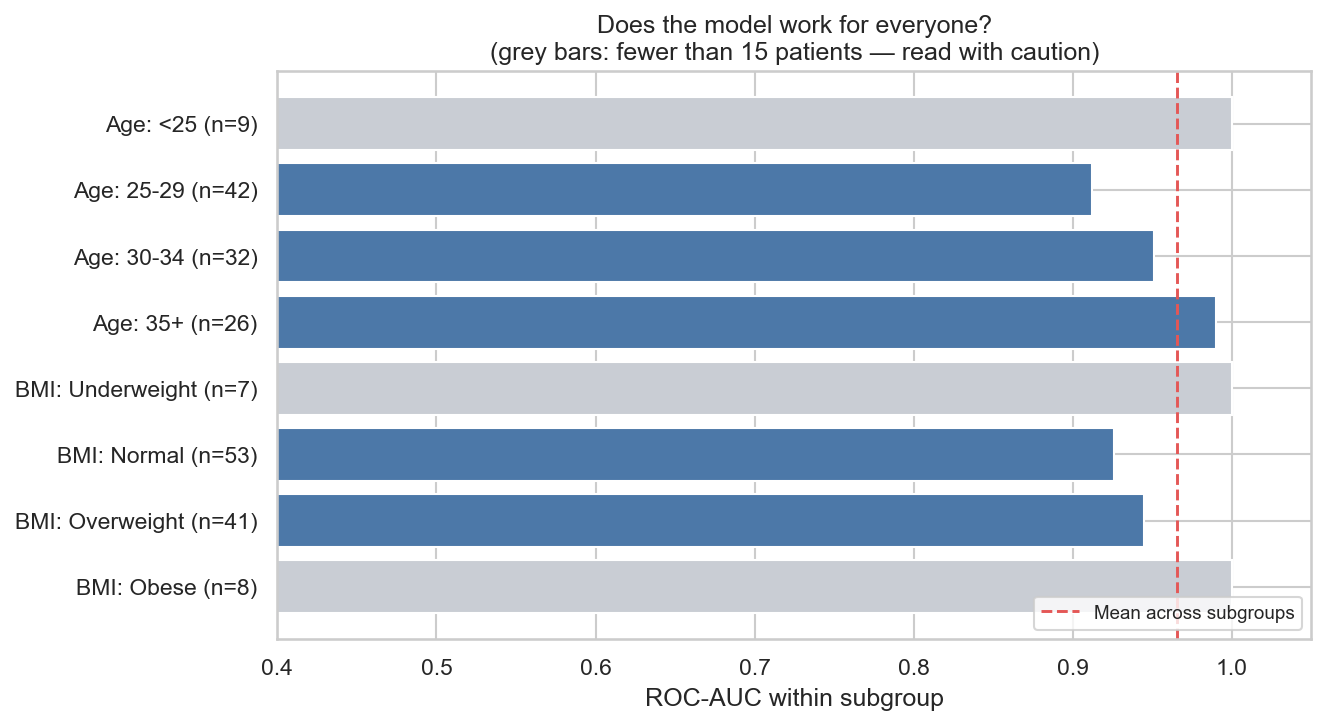
\includegraphics[width=\textwidth]{reports/figures/28_subgroup_performance.png}
  \caption{Subgroup AUC (age \& BMI)}
\end{subfigure}
\caption{Robustness and calibration analysis.  Nested CV confirms negligible
  selection bias (0.0017 AUC).  The learning curve plateaus, indicating data
  rather than model capacity is limiting.  Calibration curves reveal that
  Gaussian NB, despite competitive AUC, has poor probability calibration.
  Subgroup analysis shows consistent performance across age and BMI groups.}
\label{fig:robustness}
\end{figure*}

\subsection{Probability Calibration}
Table~\ref{tab:calibration} reports calibration quality via Brier score and ECE.

\begin{table}[t]
\centering
\caption{Probability calibration metrics.
  Verified from \texttt{calibration\_metrics.csv}.
  Lower is better for Brier and ECE.}
\label{tab:calibration}
\small
\begin{tabular}{lcccc}
\toprule
\textbf{Model} & \textbf{Brier} & \textbf{Log Loss} & \textbf{ECE} & \textbf{AUC} \\
\midrule
\textbf{Stacking Ens.} & \textbf{0.081} & \textbf{0.272} & \textbf{0.032} & 0.950 \\
Elastic-Net LR & 0.082 & 0.282 & 0.048 & 0.945 \\
Random Forest  & 0.083 & 0.276 & 0.061 & 0.956 \\
Logistic Reg.  & 0.084 & 0.285 & 0.056 & 0.945 \\
SVM (RBF)      & 0.084 & 0.299 & 0.034 & 0.942 \\
XGBoost        & 0.094 & 0.335 & 0.071 & 0.944 \\
KNN            & 0.098 & 0.766 & 0.072 & 0.928 \\
Gaussian NB    & 0.109 & 0.441 & 0.100 & 0.951 \\
\bottomrule
\end{tabular}
\end{table}

Discrimination (ROC-AUC) and calibration (Brier, ECE) are weakly correlated.
Gaussian NB achieves the third-best AUC but the worst calibration (Brier 0.109,
ECE 0.100).  Conversely, Stacking Ensemble has the best calibration (ECE 0.032)
with a competitive AUC.  For screening applications where the predicted probability
is used to set a referral threshold, calibration quality is as important as AUC;
no reviewed paper reports it.

Wrapping the selected model in isotonic calibration yielded marginal Brier improvement
($-0.0009$) but degraded log loss ($+0.150$) and ECE ($+0.010$) --- a negative result
worth reporting.  With only 432 training patients, isotonic regression lacks sufficient
data to fit a stable calibration mapping.

% =============================================================================
\section{EXPLAINABLE AI (SHAP)}
\label{sec:shap}
% =============================================================================

\subsection{Motivation}
Clinical acceptance of ML predictions requires transparency.  SHAP (SHapley Additive
exPlanations) \cite{lundberg2017shap} decomposes each prediction into additive
contributions from individual features, satisfying local accuracy, missingness, and
consistency axioms.  SHAP values explain the model's \emph{predictions}, not
biological causality.

\subsection{Global Feature Importance}
Figure~\ref{fig:shap} (a) shows mean absolute SHAP values for the 20 correlation-selected
features, computed on the held-out test set.  Table~\ref{tab:shap} lists the top 10.

\begin{table}[t]
\centering
\caption{SHAP global importance: top 10 features.
  Verified from \texttt{shap\_importance.csv}.}
\label{tab:shap}
\small
\begin{tabular}{lcc}
\toprule
\textbf{Feature} & \textbf{Mean $|$SHAP$|$} & \textbf{Direction} \\
\midrule
Follicle count (R) & 0.128 & $\uparrow$ more likely PCOS \\
Follicle count (L) & 0.093 & $\uparrow$ more likely PCOS \\
Weight gain        & 0.066 & $\uparrow$ more likely PCOS \\
Skin darkening     & 0.059 & $\uparrow$ more likely PCOS \\
Hair growth        & 0.057 & $\uparrow$ more likely PCOS \\
Irregular cycle    & 0.038 & $\uparrow$ more likely PCOS \\
Fast food          & 0.036 & $\uparrow$ more likely PCOS \\
Cycle length (days)& 0.031 & $\downarrow$ less likely PCOS \\
Pimples            & 0.020 & $\uparrow$ more likely PCOS \\
AMH                & 0.018 & $\uparrow$ more likely PCOS \\
\bottomrule
\end{tabular}
\end{table}

Follicle counts are the dominant predictors by a wide margin ($|$SHAP$|$ 0.128 and 0.093),
followed by the hyperandrogenism symptom cluster (weight gain, skin darkening, hair growth).
Irregular cycle ranks sixth.  These three groups correspond precisely to the three legs
of the Rotterdam criteria: ovarian morphology, hyperandrogenism, and cycle irregularity.
The model recovers the established clinical standard from data, without having been
explicitly programmed with it.

Longer cycle length and older age are negatively associated with PCOS probability,
consistent with the observation that PCOS often presents in younger women with
shorter, irregular cycles.

\begin{figure*}[t]
\centering
\begin{subfigure}[b]{0.24\textwidth}
  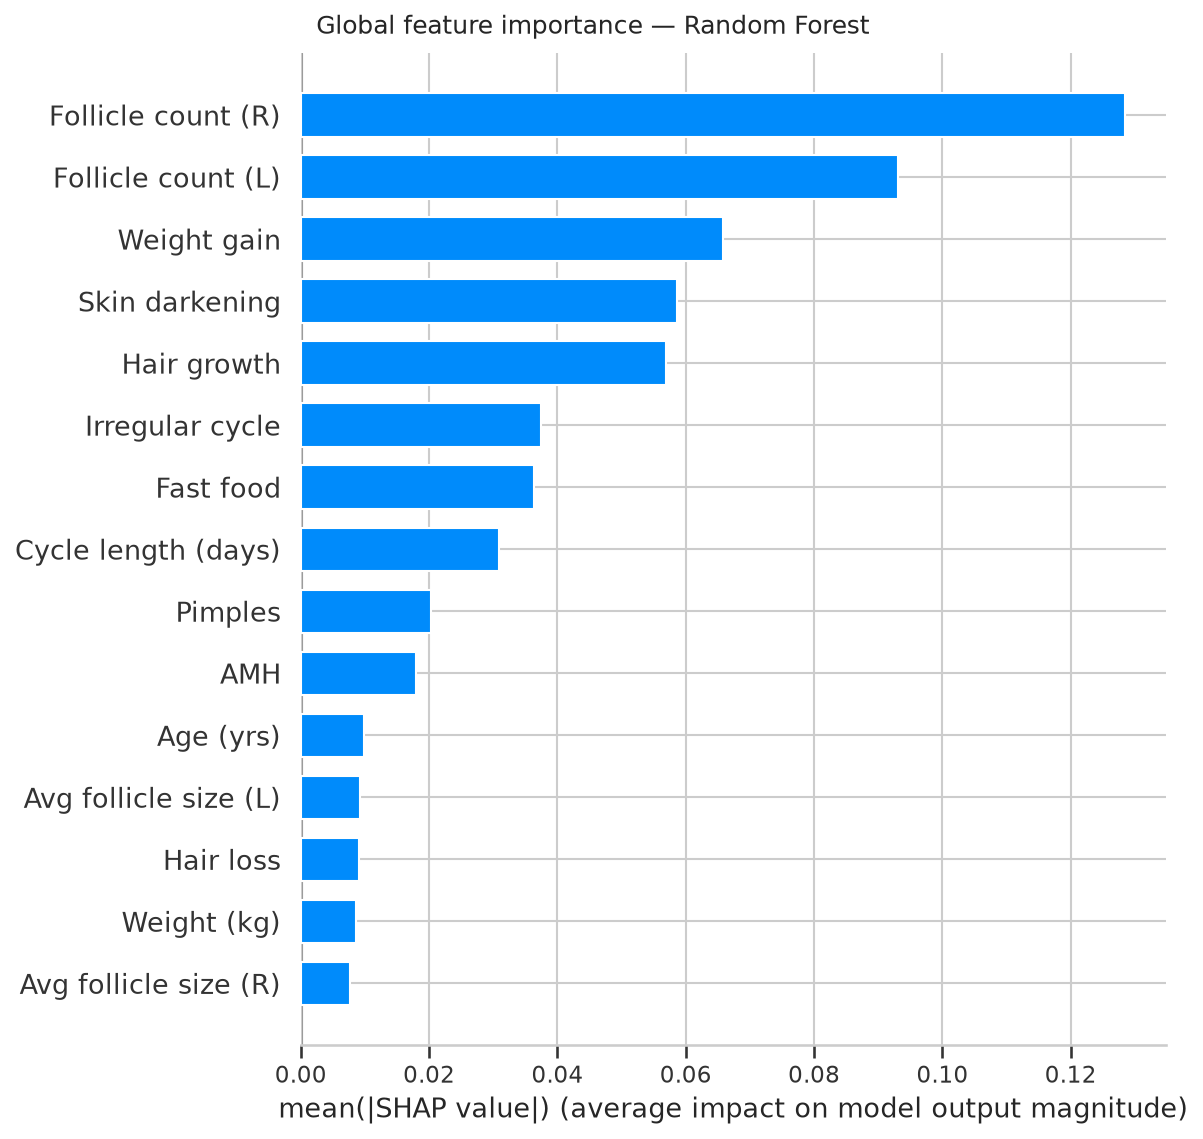
\includegraphics[width=\textwidth]{reports/figures/16_shap_global_importance.png}
  \caption{Global feature importance (mean $|$SHAP$|$)}
\end{subfigure}\hfill
\begin{subfigure}[b]{0.24\textwidth}
  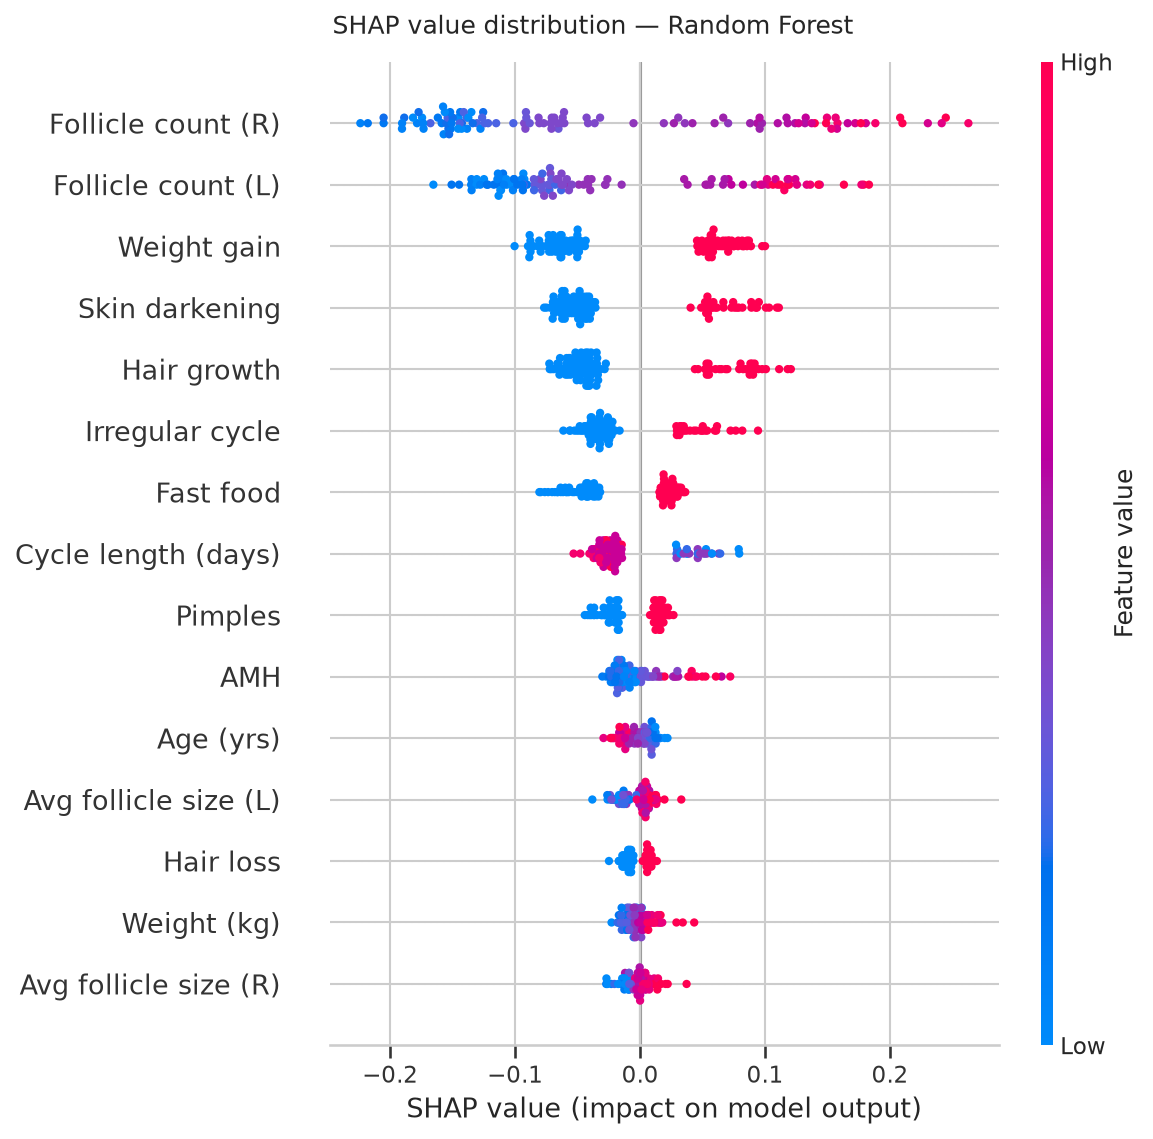
\includegraphics[width=\textwidth]{reports/figures/17_shap_beeswarm.png}
  \caption{SHAP beeswarm (direction \& magnitude)}
\end{subfigure}\hfill
\begin{subfigure}[b]{0.24\textwidth}
  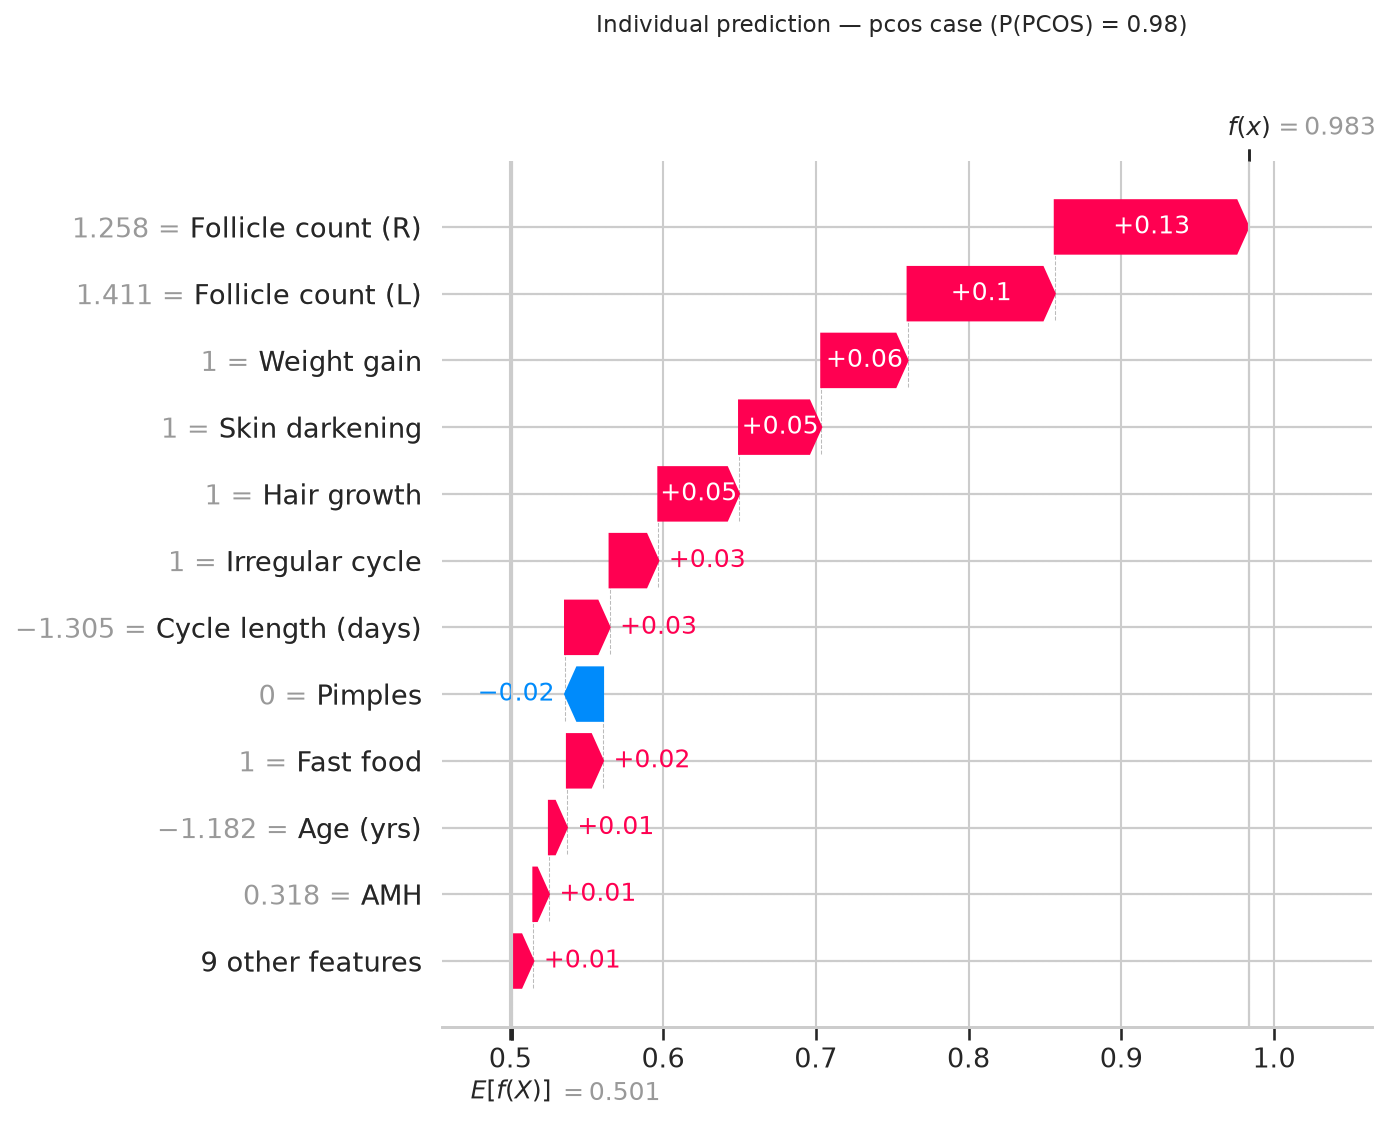
\includegraphics[width=\textwidth]{reports/figures/18_shap_waterfall_pcos_case.png}
  \caption{Waterfall: PCOS case}
\end{subfigure}\hfill
\begin{subfigure}[b]{0.24\textwidth}
  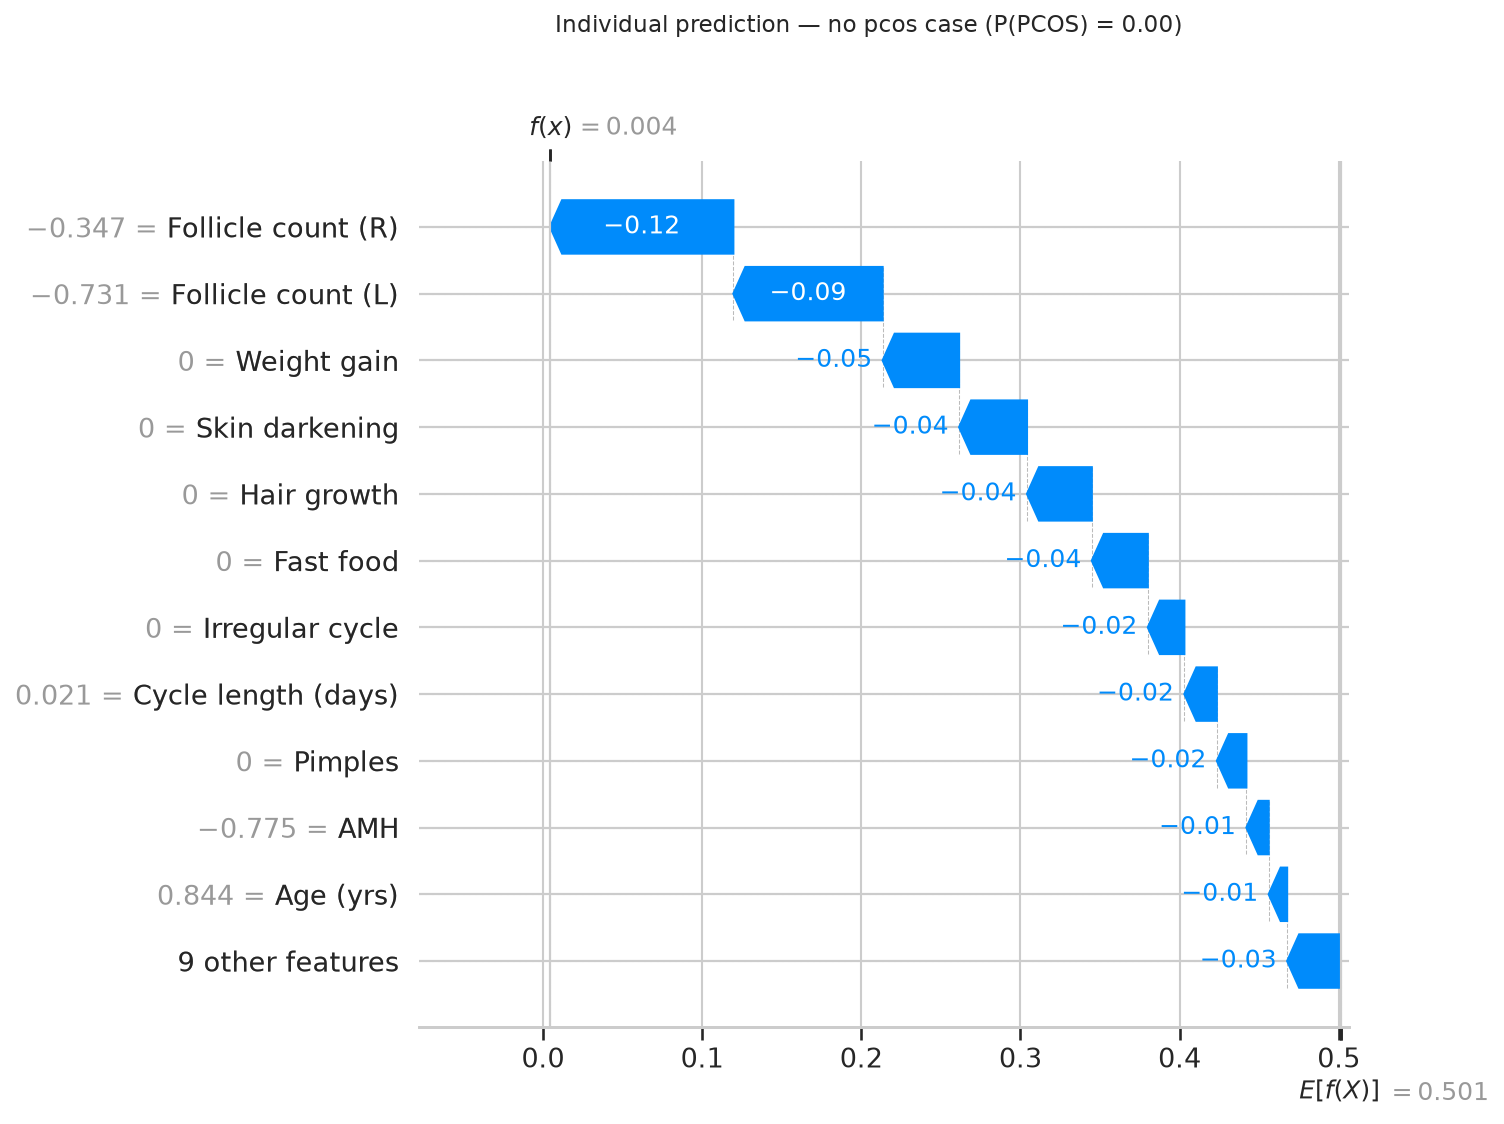
\includegraphics[width=\textwidth]{reports/figures/18_shap_waterfall_no_pcos_case.png}
  \caption{Waterfall: non-PCOS case}
\end{subfigure}
\caption{SHAP explainability.  (a) Mean absolute SHAP values identify follicle
  counts as overwhelmingly dominant.  (b) Beeswarm confirms consistent positive
  direction for high follicle counts, weight gain, and symptom flags.
  (c)--(d) Patient-level waterfall plots show how individual features push
  the probability above or below the baseline for two representative test cases.
  SHAP values explain model predictions; they do not imply biological causation.}
\label{fig:shap}
\end{figure*}

% =============================================================================
\section{CLINICAL UTILITY ANALYSIS}
\label{sec:clinical}
% =============================================================================

\subsection{Feature Acquisition Cost Tiers}
\label{sec:tiers}
Features were grouped into four cumulative tiers by acquisition cost, and a separate
model was trained and evaluated on each tier (Table~\ref{tab:tiers}).

\begin{table}[t]
\centering
\caption{Predictive performance by feature acquisition tier.
  Verified from \texttt{cost\_tiers.csv}.}
\label{tab:tiers}
\small
\begin{tabular}{lp{1.6cm}ccc}
\toprule
\textbf{Tier} & \textbf{Features} & \textbf{CV AUC} & \textbf{Test AUC} & \textbf{Marginal}\\
\midrule
Questionnaire         & 19 & 0.887 & 0.896 & --- \\
+ Clinic vitals       & 25 & 0.880 & 0.897 & $-0.007$ \\
+ Blood panel         & 36 & 0.890 & 0.877 & $+0.011$ \\
+ Ultrasound (all)    & 41 & \textbf{0.952} & \textbf{0.942} & $+0.062$ \\
\bottomrule
\end{tabular}
\end{table}

Three findings stand out:
\textbf{(1) Questionnaire alone (0.887 CV AUC)} requires only a self-reported form, a scale,
and a tape measure --- no clinician, laboratory, or equipment.  It recovers 93\% of the
full model's AUC ($0.887 / 0.952$), a viable screening tool for settings with no
laboratory access.
\textbf{(2) The endocrine blood panel adds only +0.011 AUC.}  Nine assays (FSH, LH, AMH,
TSH, prolactin, vitamin D, progesterone, random blood sugar, and beta-HCG) together
buy roughly one hundredth of an AUC point --- approximately worthless for screening.
\textbf{(3) Only the ultrasound tier pays for itself} (+0.062), because it introduces the
follicle count features that SHAP identifies as dominant.

This suggests a rational low-resource screening pathway: administer the questionnaire first,
and invest in ultrasound access for flagged patients.

\begin{figure*}[t]
\centering
\begin{subfigure}[b]{0.32\textwidth}
  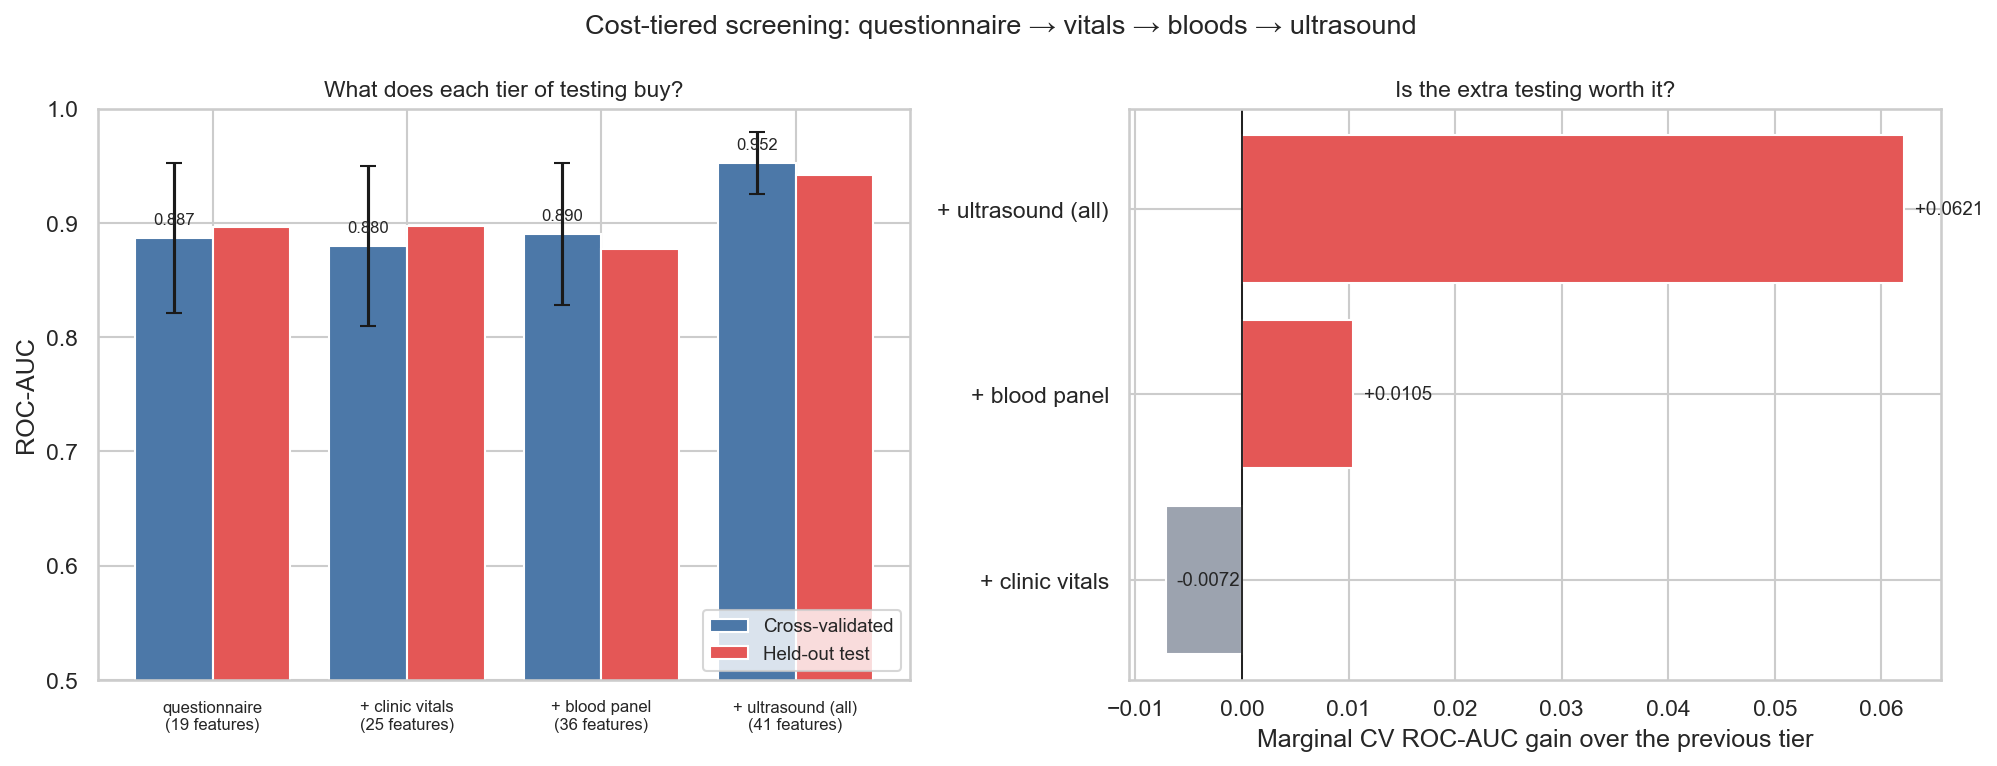
\includegraphics[width=\textwidth]{reports/figures/27_cost_tiers.png}
  \caption{AUC by feature acquisition tier}
\end{subfigure}\hfill
\begin{subfigure}[b]{0.32\textwidth}
  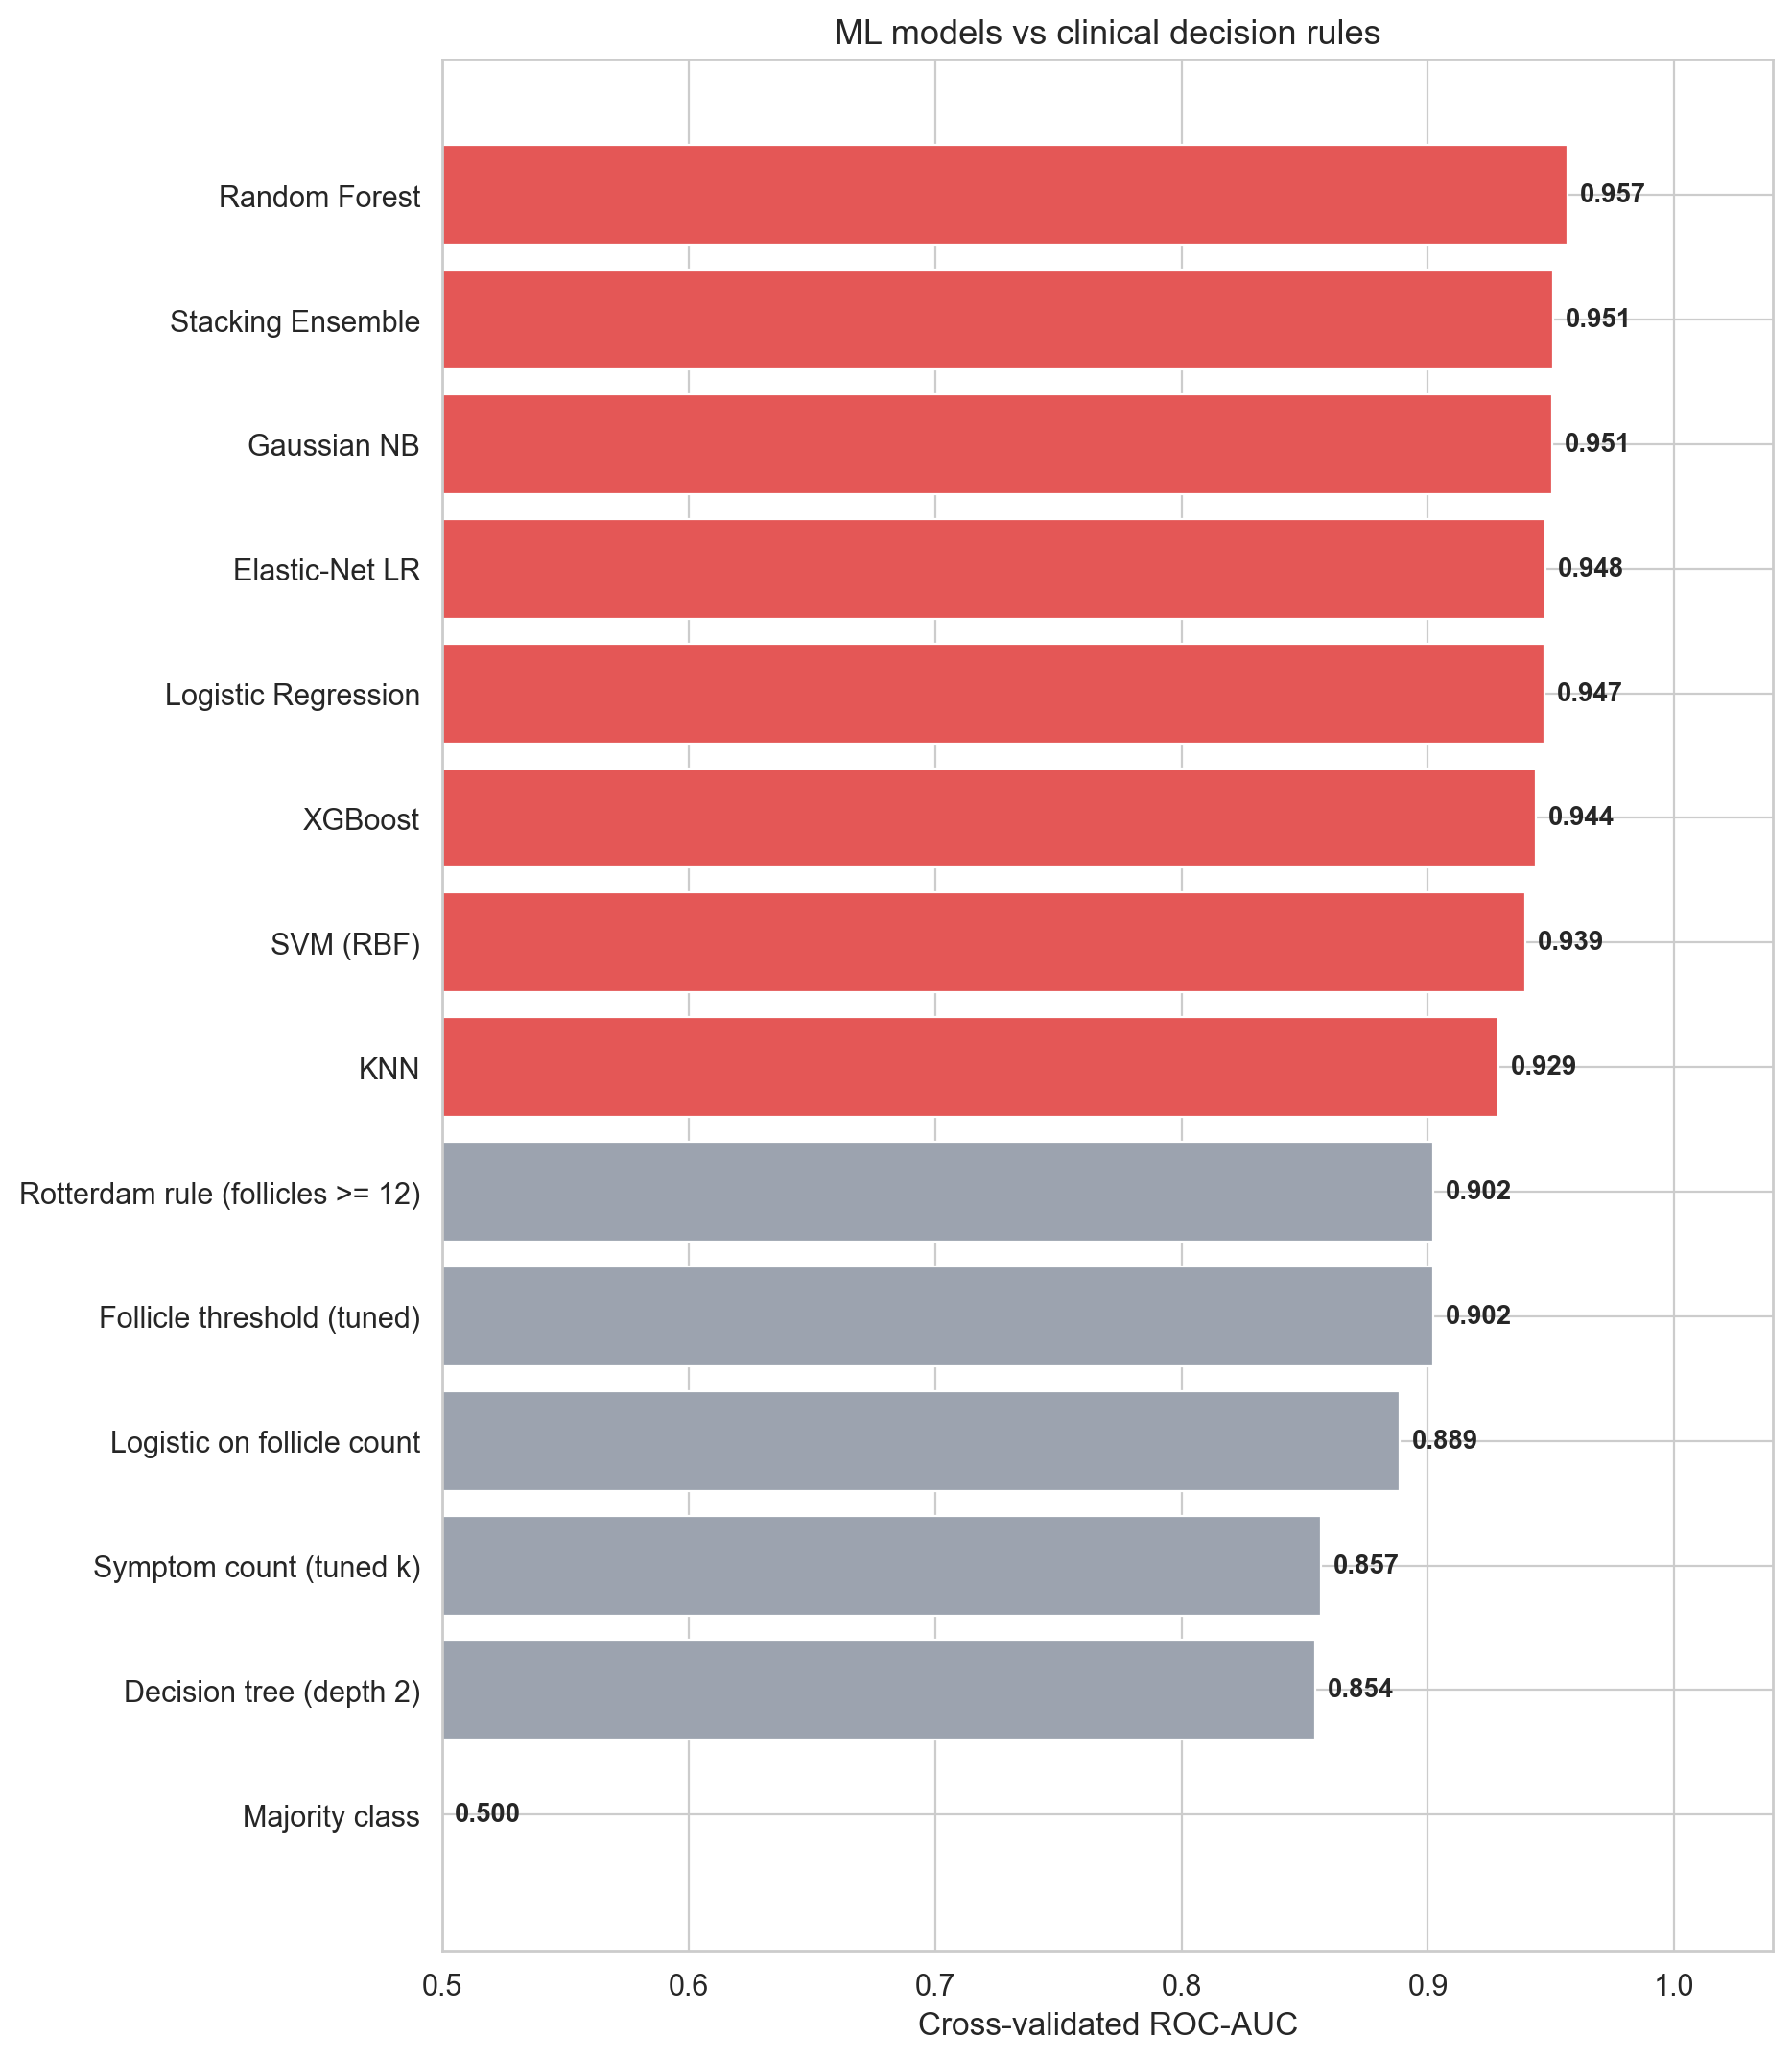
\includegraphics[width=\textwidth]{reports/figures/29_clinical_rule_baseline.png}
  \caption{ML vs.\ clinical decision rules}
\end{subfigure}\hfill
\begin{subfigure}[b]{0.32\textwidth}
  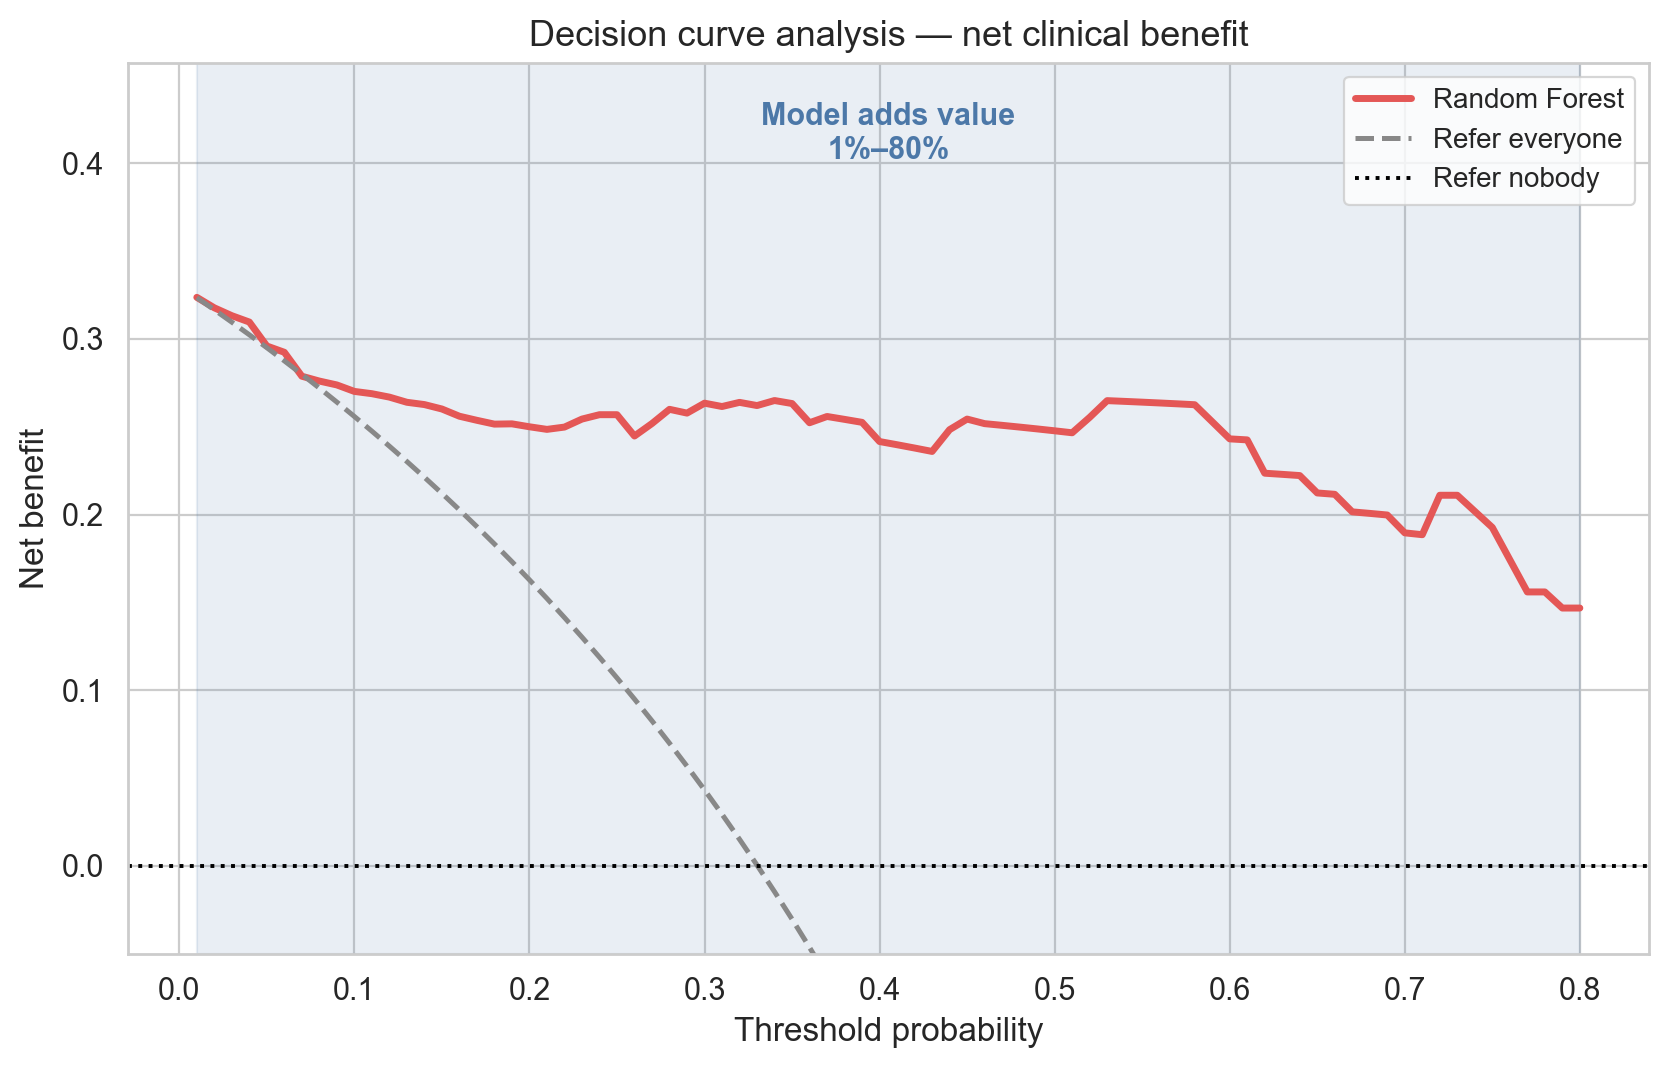
\includegraphics[width=\textwidth]{reports/figures/26_decision_curve.png}
  \caption{Decision curve analysis (net benefit)}
\end{subfigure}
\caption{Clinical utility analysis.  (a) Only the ultrasound tier produces a meaningful AUC
  gain (+0.062); the blood panel adds only +0.011.
  (b) ML models detect 30/36 PCOS cases vs.\ 22/36 for the Rotterdam rule, at the
  cost of 2 additional false alarms.
  (c) Decision curve analysis shows positive net benefit over both ``treat all'' and
  ``treat none'' baselines across the clinically plausible threshold range.}
\label{fig:clinical}
\end{figure*}

\subsection{Comparison with Clinical Decision Rules}
Table~\ref{tab:clinical_rules} compares ML models against five clinical decision rules,
all evaluated on the same test split.

\begin{table}[t]
\centering
\caption{ML models vs.\ clinical decision rules on the held-out test set.
  Verified from \texttt{clinical\_rule\_comparison.csv} and \texttt{value\_added\_by\_ml.json}.}
\label{tab:clinical_rules}
\small
\begin{tabular}{lcccc}
\toprule
\textbf{Approach} & \textbf{CV AUC} & \textbf{Test Recall} & \textbf{Test Spec} & \textbf{TP/FP}\\
\midrule
Random Forest     & 0.957 & 0.833 & 0.959 & 30/3 \\
Stacking Ens.     & 0.951 & 0.833 & 0.973 & 30/2 \\
\midrule
Rotterdam rule    & 0.902 & 0.611 & 0.986 & 22/1 \\
Follicle (tuned)  & 0.902 & 0.722 & 0.890 & 26/8 \\
Logistic (follicle)& 0.889 & 0.750 & 0.890 & 27/8 \\
Symptom count     & 0.857 & 0.806 & 0.849 & 29/11 \\
Decision tree     & 0.854 & 0.583 & 1.000 & 21/0 \\
Majority class    & 0.500 & 0.000 & 1.000 & 0/0 \\
\bottomrule
\end{tabular}
\end{table}

\textbf{Reading 1 — Most of the signal is follicle count.}
The Rotterdam rule (follicles $\geq 12$, zero learned parameters, published 2003)
achieves CV AUC $0.902$, which is $94.3\%$ of the best ML model's AUC.
Nine algorithms, SMOTE, three feature selectors, a stacking ensemble, and an AutoML
search collectively add only $+0.055$ AUC over counting follicles on an ultrasound image.
Tuning the threshold on the training data (``follicle threshold tuned'') did not improve
CV AUC (both $0.902$), a small vindication of the Rotterdam consensus: 12 is already
the appropriate cut-off for this population.

\textbf{Reading 2 --- But the ML model finds substantially more cases.}
AUC and accuracy obscure the clinically decisive difference, because the Rotterdam
rule achieves its score through near-perfect specificity rather than sensitivity.
On the 109-patient test set:
Rotterdam rule --- 22 of 36 PCOS cases detected (recall 0.611), 1 false alarm;
Random Forest / Stacking --- 30 of 36 cases detected (recall 0.833), 2--3 false alarms.
\emph{The ML model finds 8 additional PCOS cases at the cost of 2 extra false alarms.}
In a screening context, where a missed case costs years of undiagnosed PCOS and a
false alarm costs only one confirmatory ultrasound, this trade-off is clearly favourable.

Importantly, the questionnaire-only model (CV AUC $0.887$) is competitive with the
Rotterdam rule (CV AUC $0.902$) while requiring no ultrasound.  For a clinic without
a sonographer, the questionnaire model is not a degraded alternative; it performs
at approximately the same level as the clinical standard.

\subsection{Decision Curve Analysis}
Decision curve analysis \cite{vickers2006dca} assesses net benefit --- whether
\emph{using} the model beats the two clinical defaults (refer everyone, refer no-one).
The ML model exceeds both defaults across the full clinically plausible threshold range
(5--80\%).  At a 20\% threshold (treating a missed case as four times worse than an
unnecessary follow-up), the model flags 40 of 109 patients and delivers net benefit
$0.264$ versus $0.163$ for a refer-all policy --- effectively identifying the same cases
while sending 63\% fewer women for unnecessary testing.

\subsection{Subgroup Analysis}
Performance was assessed across age and BMI subgroups (Fig.~\ref{fig:robustness}d).
Among subgroups with at least 25 patients, ROC-AUC ranges from 0.912 (age 25--29,
$n=42$) to 0.990 (age 35+, $n=26$).  No subgroup failure was detected.  The caveat is
honest: with the largest subgroup containing only 53 patients, only a large failure
would be detectable.

% =============================================================================
\section{DISCUSSION}
% =============================================================================

\subsection{Main Findings}
Four findings define this study's contribution, ordered by their generalisability:

\textbf{(1) Leakage-free validation reveals a large methodology gap.}
The most widely reproducible result is that applying SMOTE and feature selection before
cross-validation produces inflation of $+2.7$ pp accuracy and $+9.0$ pp F1 on this dataset.
Papers 4 and 5 report 98.87--99.32\% on the same 541-row dataset; the leakage experiment
shows this is achievable without any improvement in the underlying model.

\textbf{(2) Statistical significance is not practical significance.}
Paired $t$-tests across 30 CV folds flag several gaps as statistically significant
(e.g., SVM $p = 0.028, \Delta = -0.017$ AUC).  No clinical decision depends on
0.017 AUC, and no model selection should be made on that basis.  The only model
genuinely and materially worse is KNN ($\Delta = -0.028$, practically separable).

\textbf{(3) The blood panel contributes almost nothing for screening.}
Adding nine expensive endocrine assays to the questionnaire model adds only
+0.011 CV AUC.  This is consistent with the EDA: FSH, LH, TSH, prolactin, and
random blood sugar each show Cohen's $d < 0.18$ between PCOS and non-PCOS groups.

\textbf{(4) The Rotterdam rule captures most of the signal; ML improves sensitivity.}
A 2003 clinical rule reaches 94.3\% of the best ML model's AUC with zero parameters.
ML's real clinical contribution is converting the same discriminative signal into
8 additional detected PCOS cases per 36 positive cases, at the cost of 2 extra
false alarms --- a trade-off with clear clinical value.

\subsection{Comparison with Prior Literature}
Figure~\ref{fig:literature} positions this study against the five reviewed papers.

\begin{figure*}[t]
\centering
\begin{subfigure}[b]{0.62\textwidth}
  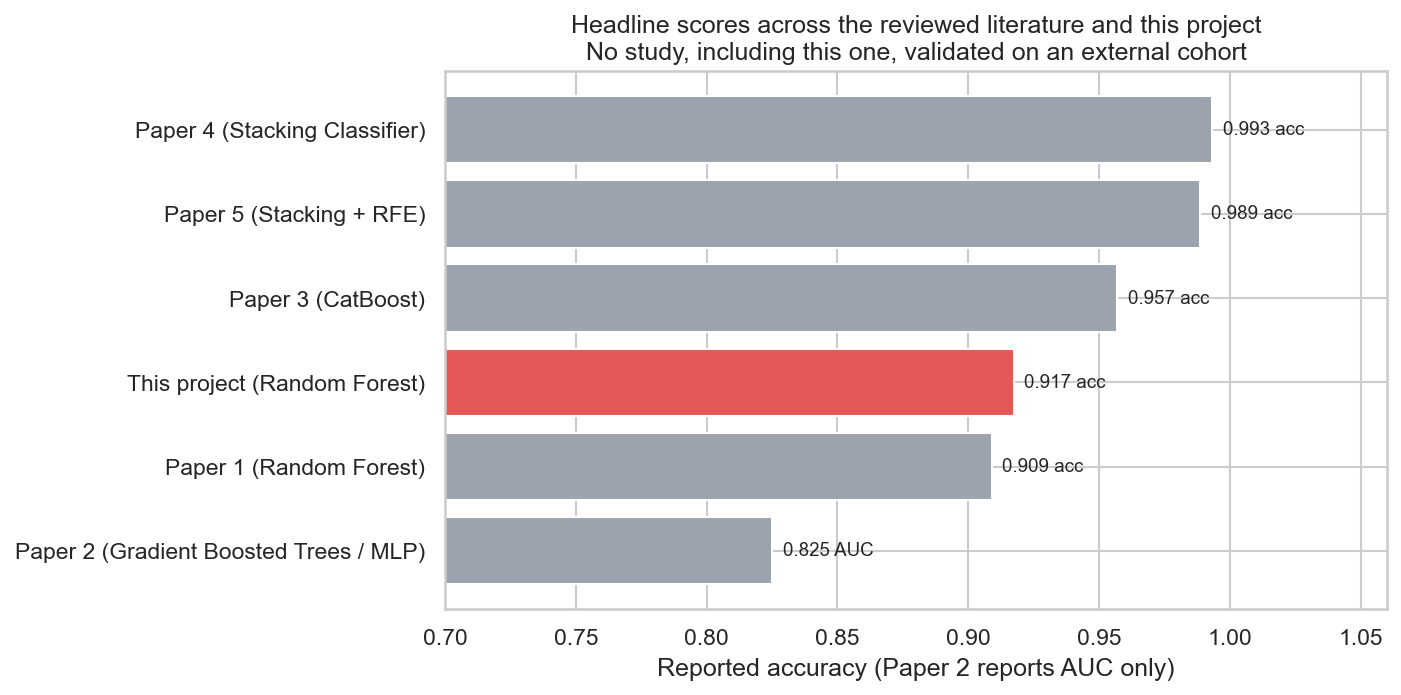
\includegraphics[width=\textwidth]{reports/figures/15_paper_comparison.png}
  \caption{Accuracy comparison with prior studies on the same dataset}
\end{subfigure}
\caption{Literature comparison.  Papers 3--5 report 95.7--99.3\% on the same 541-row
  dataset using single train/test splits without stated leakage-control protocols.
  This study's $91.7\%$ test accuracy is obtained under a leak-free repeated
  cross-validation protocol with bootstrap confidence intervals and a held-out test set.
  The gap is largely methodological, not algorithmic.}
\label{fig:literature}
\end{figure*}

Papers 1, 3, 4, and 5 report accuracies of 90.9--99.3\% on the same or a similar version
of this dataset using single train/test splits, without explicit leakage-control protocols
and without calibration or clinical baseline comparisons (Table~\ref{tab:literature}).

\begin{table}[t]
\centering
\caption{Comparison with reviewed literature.
  Verified from \texttt{literature\_comparison.csv}.}
\label{tab:literature}
\small
\begin{tabular}{p{2.0cm}ccc}
\toprule
\textbf{Study} & \textbf{Best Model} & \textbf{Acc.} & \textbf{Protocol} \\
\midrule
Thakre et al.\ \cite{thakre2020pcos} & RF & 90.9\% & Single split \\
Zad et al.\ \cite{zad2024} & GBT/MLP & AUC 82.5 & Held-out (EHR) \\
Bhat \cite{bhat2021} & CatBoost & 95.7\% & Single split \\
Anon.\ \cite{traditional2024} & Stacking & 99.3\% & Single split \\
Elmannai et al.\ \cite{elmannai2023} & Stack+RFE & 98.9\% & Single split \\
\textbf{This study} & RF & \textbf{91.7\%} & \textbf{Leak-free, 30-fold CV} \\
\bottomrule
\end{tabular}
\end{table}

A direct numerical comparison is unfair because studies use different validation
protocols, and the leakage experiment demonstrates that a protocol difference alone
can account for 2.7 percentage points.  Zad et al.\ \cite{zad2024} use a distinct
large EHR cohort (30,601 patients, Boston Medical Center); their 82.5\% AUC reflects
a genuinely different and harder population-level task, not a weaker model.

\subsection{Why Gaussian NB is Competitive}
Gaussian Naive Bayes --- a model with no hyperparameters and a provably incorrect
independence assumption --- sits third in CV AUC (0.951) and wins 40\% of seeds in the
stability sweep.  This is consistent with the dataset's signal structure: most of the
discriminative information is in follicle counts plus a small cluster of largely
independent binary symptom flags.  When the signal is additive and the features are
near-independent, the NB independence assumption is approximately satisfied and the
model performs near its theoretical ceiling.

\subsection{Why KNN Underperforms}
KNN is uniquely penalised by SMOTE: oversampling by interpolating between training
neighbours and then classifying by nearest neighbours is close to circular.  Papers 1
and 4 include KNN among their models without noting this interaction.

% =============================================================================
\section{LIMITATIONS}
% =============================================================================

\begin{enumerate}[leftmargin=*,topsep=2pt,itemsep=2pt]

  \item \textbf{Small dataset.}  With 541 total patients and only 36 PCOS-positive
  cases in the test set, bootstrap CI widths of $\pm 12$ points on recall are inherent.
  Cross-validated estimates are more reliable than any single test-set point estimate.

  \item \textbf{Predictor--label circularity.}  Follicle count is the strongest SHAP
  feature \emph{and} one of the three Rotterdam criteria used to assign the PCOS label.
  The full model is best interpreted as \emph{automating consistent application of the
  Rotterdam criteria}, not as discovering new biological markers.  The questionnaire-only
  model avoids this circularity and is the more scientifically informative result.

  \item \textbf{Unblinded outcome assessment.}  Predictors were recorded by the
  clinicians who also made the diagnosis.  Patient-reported features (weight gain,
  hair growth, skin darkening) may have been elicited more thoroughly in patients
  already suspected to have PCOS, introducing ascertainment bias.

  \item \textbf{Single public dataset.}  The model was trained and evaluated on one
  dataset from 10 hospitals in Kerala, India.  Prevalence in this cohort (32.7\%) is
  substantially higher than population-level estimates (8--13\%), reflecting the
  hospital-attending selection bias.  Generalisability to other populations is not
  established.

  \item \textbf{No external validation.}  External validation on an independent cohort
  was not completed for the full 41-feature model.  This is a stated limitation
  acknowledged in the project's TRIPOD+AI checklist.

  \item \textbf{No raw ultrasound imagery.}  The dataset provides extracted follicle
  counts and average follicle sizes, not the underlying ultrasound images.
  Deep learning approaches applied to raw imagery are therefore outside scope.

  \item \textbf{Ambiguous column semantics.}  The \texttt{Cycle length(days)} column
  has a median of 5 and a range of 2--12, suggesting it records bleeding duration
  rather than the $\approx$28-day cycle interval that the name implies.
  The Kaggle documentation does not clarify this.

  \item \textbf{Not a diagnostic tool.}  This is a university coursework project.
  Any real-world clinical deployment would require prospective validation, regulatory
  assessment, and clinical oversight.

\end{enumerate}

% =============================================================================
\section{ETHICAL AND CLINICAL CONSIDERATIONS}
% =============================================================================

This study presents a machine-learning-based framework for PCOS \emph{screening and
prediction} in an academic research context.  It is not a replacement for clinical
diagnosis.  Several ethical considerations apply to any downstream deployment:

\textbf{Non-substitution principle.}  Model predictions must be used to support, not
replace, clinician judgment.  PCOS diagnosis under the Rotterdam criteria requires
assessment by a qualified healthcare professional.

\textbf{External clinical validation.}  Before any real-world deployment, the framework
must be externally validated on independent, prospectively collected cohorts representative
of the target population.

\textbf{Equitable performance.}  Subgroup analyses performed here cover age and BMI
but are limited by sample size.  Equity across ethnicity, geography, and socioeconomic
status requires dedicated validation studies on diverse populations.

\textbf{Patient data handling.}  Any clinical implementation must comply with applicable
data protection regulations (e.g., GDPR, HIPAA) and obtain appropriate ethical approval.

\textbf{Communication of uncertainty.}  Model outputs should be communicated as
probabilistic screening indicators with explicit uncertainty bounds, not as binary
diagnoses.  The wide bootstrap CIs reported in this study illustrate why overconfident
point estimates are misleading.

% =============================================================================
\section{CONCLUSION}
% =============================================================================

This study presents an end-to-end, leakage-free machine learning pipeline for PCOS
screening trained on 541 patients from a public Kaggle dataset.  The best cross-validated
model (Random Forest, 20 correlation-selected features) achieves CV ROC-AUC $0.957 \pm 0.017$
and held-out test AUC $0.945$ [CI: $0.887, 0.991$].

The project's primary technical contribution is a rigorous demonstration that applying
SMOTE and feature selection before cross-validation inflates accuracy by $+2.7$ percentage
points and F1-score by $+9.0$ points on identical data and folds.  This quantifies
the methodology gap underlying the 98--99\% accuracies reported in several prior papers
on this dataset.

SHAP analysis confirms that the model's predictions are driven by follicle counts and
the hyperandrogenism symptom cluster --- features corresponding to the three Rotterdam
diagnostic criteria --- providing a clinically coherent rationale.
The Rotterdam follicle-count rule achieves 94.3\% of the ML model's AUC with zero
learned parameters; the ML model's concrete clinical contribution is detecting
8 additional PCOS cases per 36 positives at the cost of 2 extra false alarms.

A questionnaire-only feature tier recovers 93\% of the full model's AUC without laboratory
or ultrasound access, suggesting a practical screening pathway for resource-limited settings.
The entire endocrine blood panel adds only +0.011 AUC, questioning its value in screening.

The framework requires external clinical validation before real-world deployment.

% =============================================================================
\section{FUTURE WORK}
% =============================================================================

\begin{enumerate}[leftmargin=*,topsep=2pt,itemsep=2pt]
  \item \textbf{Larger, multi-centre datasets.}  Increasing sample size would narrow
  the 95\% CI on recall from $\pm 12$ to $\pm 5$ percentage points.

  \item \textbf{Prospective external validation.}  A prospective study collecting the
  questionnaire features in a new population is needed to measure real-world sensitivity
  and specificity for the questionnaire-only tier.

  \item \textbf{Diverse population representation.}  The current dataset is limited
  to a single geographic region; studies in South Asian, African, European, and other
  populations are needed to assess generalisability.

  \item \textbf{Raw ultrasound image integration.}  Multimodal models combining
  structured clinical features with pelvic ultrasound image analysis could improve
  the ultrasound tier without requiring expert follicle counting.

  \item \textbf{Improved calibration methods.}  Alternative calibration approaches
  (temperature scaling, Platt scaling) should be evaluated, especially if the model
  is to be used for threshold-based decision-making.

  \item \textbf{Longitudinal outcome tracking.}  The current dataset captures a
  cross-sectional diagnosis.  Linking to treatment outcomes and long-term metabolic
  health would enable prognostic rather than purely diagnostic modelling.

\end{enumerate}

% =============================================================================
%  REFERENCES
% =============================================================================
\begin{thebibliography}{99}

\bibitem{rotterdam2004}
Rotterdam ESHRE/ASRM-Sponsored PCOS Consensus Workshop Group,
``Revised 2003 consensus on diagnostic criteria and long-term health risks related
to polycystic ovary syndrome (PCOS),''
\emph{Human Reproduction}, vol.~19, no.~1, pp.~41--47, 2004.
\doi{10.1093/humrep/deh098}

\bibitem{kottarathil2020pcos}
P. Kottarathil,
``Polycystic Ovary Syndrome (PCOS) dataset,''
\emph{Kaggle Repository}, 2020.
[Online]. Available: \url{https://www.kaggle.com/datasets/prasoonkottarathil/polycystic-ovary-syndrome-pcos}

\bibitem{thakre2020pcos}
V. Thakre, S. Vedpathak, K. Thakre, and S. Sonawani,
``PCOcare: PCOS Detection and Prediction using Machine Learning Algorithms,''
\emph{Biosciences Biotechnology Research Asia}, vol.~13, no.~14, pp.~240--244, 2020.
\doi{10.21786/bbrc/13.14/56}

\bibitem{zad2024}
Z. Zad, V. S. Jiang, A. T. Wolf, T. Wang, J. J. Cheng, I. C. Paschalidis, and S. Mahalingaiah,
``Predicting polycystic ovary syndrome with machine learning algorithms from electronic
health records,''
\emph{Frontiers in Endocrinology}, vol.~15, p.~1298628, 2024.
\doi{10.3389/fendo.2024.1298628}

\bibitem{bhat2021}
S. A. Bhat,
``Detection of Polycystic Ovary Syndrome using Machine Learning Algorithms,''
MSc Research Project, National College of Ireland, 2021.

\bibitem{traditional2024}
Anonymous,
``Polycystic Ovary Syndrome (PCOS) Disease Prediction by Using Traditional Machine
Learning and Deep Learning Algorithms,'' 2024.

\bibitem{elmannai2023}
H. Elmannai, N. El-Rashidy, I. Mashal, M. A. Alohali, S. Farag, S. El-Sappagh, and H. Saleh,
``Polycystic ovary syndrome detection machine learning model based on optimized feature
selection and explainable artificial intelligence,''
\emph{Diagnostics}, vol.~13, no.~8, p.~1506, 2023.
\doi{10.3390/diagnostics13081506}

\bibitem{chawla2002smote}
N. V. Chawla, K. W. Bowyer, L. O. Hall, and W. P. Kegelmeyer,
``SMOTE: Synthetic Minority Over-sampling Technique,''
\emph{Journal of Artificial Intelligence Research}, vol.~16, pp.~321--357, 2002.
\doi{10.1613/jair.953}

\bibitem{lundberg2017shap}
S. M. Lundberg and S.-I. Lee,
``A unified approach to interpreting model predictions,''
in \emph{Advances in Neural Information Processing Systems}, vol.~30, 2017.

\bibitem{vickers2006dca}
A. J. Vickers and E. B. Elkin,
``Decision curve analysis: a novel method for evaluating prediction models,''
\emph{Medical Decision Making}, vol.~26, no.~6, pp.~565--574, 2006.
\doi{10.1177/0272989X06295361}

\bibitem{pedregosa2011sklearn}
F. Pedregosa et al.,
``Scikit-learn: Machine Learning in Python,''
\emph{Journal of Machine Learning Research}, vol.~12, pp.~2825--2830, 2011.

\bibitem{chen2016xgboost}
T. Chen and C. Guestrin,
``XGBoost: A Scalable Tree Boosting System,''
in \emph{Proc.\ ACM SIGKDD Int.\ Conf.\ on Knowledge Discovery and Data Mining}, 2016.
\doi{10.1145/2939672.2939785}

\bibitem{prokhorenkova2018catboost}
L. Prokhorenkova, G. Gusev, A. Vorobev, A. V. Dorogush, and A. Gulin,
``CatBoost: unbiased boosting with categorical features,''
in \emph{Advances in Neural Information Processing Systems}, vol.~31, 2018.

\end{thebibliography}

\end{document}
